\documentclass[a4paper,11pt,fleqn,twoside,openright]{memoir} 	% Openright aabner kapitler paa hoejresider (openany begge)

%%%% PACKAGES %%%%

% ¤¤ Oversaettelse og tegnsaetning ¤¤ %
%tilføjet af AT
\usepackage{url}
\usepackage{rotating}
\usepackage{pdflscape}

\usepackage[utf8]{inputenc}					% Input-indkodning af tegnsaet (UTF8)
\usepackage[danish]{babel}					% Dokumentets sprog
\usepackage[T1]{fontenc}					% Output-indkodning af tegnsaet (T1)
\usepackage{ragged2e,anyfontsize}			% Justering af elementer
\usepackage{fixltx2e}						% Retter forskellige fejl i LaTeX-kernen	
								\usepackage{blindtext}	
								
% ¤¤ Figurer og tabeller (floats) ¤¤ %
\usepackage{graphicx} 						% Haandtering af eksterne billeder (JPG, PNG, PDF)
\usepackage{multirow}                		% Fletning af raekker og kolonner (\multicolumn og \multirow)
\usepackage{colortbl} 						% Farver i tabeller (fx \columncolor, \rowcolor og \cellcolor)
\usepackage[dvipsnames]{xcolor}				% Definer farver med \definecolor. Se mere: http://en.wikibooks.org/wiki/LaTeX/Colors
\usepackage{flafter}						% Soerger for at floats ikke optraeder i teksten foer deres reference
\let\newfloat\relax 						% Justering mellem float-pakken og memoir
\usepackage{float}							% Muliggoer eksakt placering af floats, f.eks. \begin{figure}[H]
%\usepackage{eso-pic}						% Tilfoej billedekommandoer paa hver side
%\usepackage{wrapfig}						% Indsaettelse af figurer omsvoebt af tekst. \begin{wrapfigure}{Placering}{Stoerrelse}
%\usepackage{multicol}         	        	% Muliggoer tekst i spalter
%\usepackage{rotating}						% Rotation af tekst med \begin{sideways}...\end{sideways}
\usepackage{longtable}

% ¤¤ Matematik mm. ¤¤
\usepackage{amsmath,amssymb,stmaryrd} 		% Avancerede matematik-udvidelser
\usepackage{mathtools}						% Andre matematik- og tegnudvidelser
\usepackage{textcomp}                 		% Symbol-udvidelser (f.eks. promille-tegn med \textperthousand )
\usepackage{siunitx}						% Flot og konsistent praesentation af tal og enheder med \si{enhed} og \SI{tal}{enhed}
\sisetup{output-decimal-marker = {,}}		% Opsaetning af \SI (DE for komma som decimalseparator) 
\usepackage[version=3]{mhchem} 				% Kemi-pakke til flot og let notation af formler, f.eks. \ce{Fe2O3}
%\usepackage{rsphrase}						% Kemi-pakke til RS-saetninger, f.eks. \rsphrase{R1}

% ¤¤ Referencer og kilder ¤¤ %
\usepackage[danish]{varioref}				% Muliggoer bl.a. krydshenvisninger med sidetal (\vref)
\usepackage{natbib}							% Udvidelse med naturvidenskabelige citationsmodeller
%\usepackage{xr}							% Referencer til eksternt dokument med \externaldocument{<NAVN>}
%\usepackage{glossaries}					% Terminologi- eller symbolliste (se mere i Daleifs Latex-bog)

% ¤¤ Misc. ¤¤ %
\usepackage{listings}						% Placer kildekode i dokumentet med \begin{lstlisting}...\end{lstlisting}
\usepackage{lipsum}							% Dummy text \lipsum[..]
\usepackage[shortlabels]{enumitem}			% Muliggoer enkelt konfiguration af lister
\usepackage{pdfpages}						% Goer det muligt at inkludere pdf-dokumenter med kommandoen \includepdf[pages={x-y}]{fil.pdf}	
\pdfoptionpdfminorversion=6					% Muliggoer inkludering af pdf dokumenter, af version 1.6 og hoejere
\pretolerance=2500 							% Justering af afstand mellem ord (hoejt tal, mindre orddeling og mere luft mellem ord)

% Kommentarer og rettelser med \fxnote. Med 'final' i stedet for 'draft' udloeser hver note en error i den faerdige rapport.
\usepackage[footnote,draft,danish,silent,nomargin]{fixme}		


%%%% CUSTOM SETTINGS %%%%

% ¤¤ Marginer ¤¤ %
\setlrmarginsandblock{3.5cm}{2.5cm}{*}		% \setlrmarginsandblock{Indbinding}{Kant}{Ratio}
\setulmarginsandblock{2.5cm}{3.0cm}{*}		% \setulmarginsandblock{Top}{Bund}{Ratio}
\checkandfixthelayout 						% Oversaetter vaerdier til brug for andre pakker

%	¤¤ Afsnitsformatering ¤¤ %
\setlength{\parindent}{0mm}           		% Stoerrelse af indryk
\setlength{\parskip}{3mm}          			% Afstand mellem afsnit ved brug af double Enter
\linespread{1,1}							% Linie afstand

% ¤¤ Litteraturlisten ¤¤ %
\bibpunct[,]{[}{]}{;}{a}{,}{,} 				% Definerer de 6 parametre ved Harvard henvisning (bl.a. parantestype og seperatortegn)
\bibliographystyle{bibtex/harvard}			% Udseende af litteraturlisten.

% ¤¤ Indholdsfortegnelse ¤¤ %
\setcounter{secnumdepth}{4}		 			% Dybden af nummerede overkrifter (part/chapter/section/subsection)
\setcounter{maxsecnumdepth}{4}					% Dokumentklassens graense for nummereringsdybde
\setcounter{tocdepth}{4} 					% Dybden af indholdsfortegnelsen

% ¤¤ Lister ¤¤ %
\setlist{
  topsep=0pt,								% Vertikal afstand mellem tekst og listen
  itemsep=-1ex,								% Vertikal afstand mellem items
} 

% ¤¤ Visuelle referencer ¤¤ %
\usepackage[colorlinks]{hyperref}			% Danner klikbare referencer (hyperlinks) i dokumentet.
\hypersetup{colorlinks = true,				% Opsaetning af farvede hyperlinks (interne links, citeringer og URL)
    linkcolor = black,
    citecolor = black,
    urlcolor = black
}

% ¤¤ Opsaetning af figur- og tabeltekst ¤¤ %
\captionnamefont{\small\bfseries\itshape}	% Opsaetning af tekstdelen ('Figur' eller 'Tabel')
\captiontitlefont{\small}					% Opsaetning af nummerering
\captiondelim{. }							% Seperator mellem nummerering og figurtekst
\hangcaption								% Venstrejusterer flere-liniers figurtekst under hinanden
\captionwidth{\linewidth}					% Bredden af figurteksten
\setlength{\belowcaptionskip}{0pt}			% Afstand under figurteksten
		
% ¤¤ Opsaetning af listings ¤¤ %
\definecolor{commentGreen}{RGB}{34,139,24}
\definecolor{stringPurple}{RGB}{208,76,239}

\lstset{language=Matlab,					% Sprog
	basicstyle=\ttfamily\scriptsize,		% Opsaetning af teksten
	keywords={for,if,while,else,elseif,		% Noegleord at fremhaeve
			  end,break,return,case,
			  switch,function},
	keywordstyle=\color{blue},				% Opsaetning af noegleord
	commentstyle=\color{commentGreen},		% Opsaetning af kommentarer
	stringstyle=\color{stringPurple},		% Opsaetning af strenge
	showstringspaces=false,					% Mellemrum i strenge enten vist eller blanke
	numbers=left, numberstyle=\tiny,		% Linjenumre
	extendedchars=true, 					% Tillader specielle karakterer
	columns=flexible,						% Kolonnejustering
	breaklines, breakatwhitespace=true,		% Bryd lange linjer
}

% ¤¤ Navngivning ¤¤ %
\addto\captionsdanish{
	\renewcommand\appendixname{Appendiks}
	\renewcommand\contentsname{Indholdsfortegnelse}	
	\renewcommand\appendixpagename{Appendiks}
	\renewcommand\appendixtocname{Appendiks}
	\renewcommand\cftchaptername{\chaptername~}				% Skriver "Kapitel" foran kapitlerne i indholdsfortegnelsen
	\renewcommand\cftappendixname{\appendixname~}			% Skriver "Appendiks" foran appendiks i indholdsfortegnelsen
}

% ¤¤ Kapiteludssende ¤¤ %
\definecolor{numbercolor}{gray}{0.7}		% Definerer en farve til brug til kapiteludseende
\newif\ifchapternonum

\makechapterstyle{jenor}{					% Definerer kapiteludseende frem til ...
  \renewcommand\beforechapskip{0pt}
  \renewcommand\printchaptername{}
  \renewcommand\printchapternum{}
  \renewcommand\printchapternonum{\chapternonumtrue}
  \renewcommand\chaptitlefont{\fontfamily{pbk}\fontseries{db}\fontshape{n}\fontsize{25}{35}\selectfont\raggedleft}
  \renewcommand\chapnumfont{\fontfamily{pbk}\fontseries{m}\fontshape{n}\fontsize{1in}{0in}\selectfont\color{numbercolor}}
  \renewcommand\printchaptertitle[1]{%
    \noindent
    \ifchapternonum
    \begin{tabularx}{\textwidth}{X}
    {\let\\\newline\chaptitlefont ##1\par} 
    \end{tabularx}
    \par\vskip-2.5mm\hrule
    \else
    \begin{tabularx}{\textwidth}{Xl}
    {\parbox[b]{\linewidth}{\chaptitlefont ##1}} & \raisebox{-15pt}{\chapnumfont \thechapter}
    \end{tabularx}
    \par\vskip2mm\hrule
    \fi
  }
}											% ... her

\chapterstyle{jenor}						% Valg af kapiteludseende - Google 'memoir chapter styles' for alternativer

% ¤¤ Sidehoved ¤¤ %

\makepagestyle{Uni}							% Definerer sidehoved og sidefod udseende frem til ...
\makepsmarks{Uni}{%
	\createmark{chapter}{left}{shownumber}{}{. \ }
	\createmark{section}{right}{shownumber}{}{. \ }
	\createplainmark{toc}{both}{\contentsname}
	\createplainmark{lof}{both}{\listfigurename}
	\createplainmark{lot}{both}{\listtablename}
	\createplainmark{bib}{both}{\bibname}
	\createplainmark{index}{both}{\indexname}
	\createplainmark{glossary}{both}{\glossaryname}
}
\nouppercaseheads											% Ingen Caps oenskes

\makeevenhead{Uni}{Langerhanske Øer}{}{\leftmark}				% Definerer lige siders sidehoved (\makeevenhead{Navn}{Venstre}{Center}{Hoejre})
\makeoddhead{Uni}{\rightmark}{}{Ingeniørhøjskolen Aarhus}			% Definerer ulige siders sidehoved (\makeoddhead{Navn}{Venstre}{Center}{Hoejre})
\makeevenfoot{Uni}{\thepage}{}{}							% Definerer lige siders sidefod (\makeevenfoot{Navn}{Venstre}{Center}{Hoejre})
\makeoddfoot{Uni}{}{}{\thepage}								% Definerer ulige siders sidefod (\makeoddfoot{Navn}{Venstre}{Center}{Hoejre})
\makeheadrule{Uni}{\textwidth}{0.5pt}						% Tilfoejer en streg under sidehovedets indhold
\makefootrule{Uni}{\textwidth}{0.5pt}{1mm}					% Tilfoejer en streg under sidefodens indhold

\copypagestyle{Unichap}{Uni}								% Sidehoved for kapitelsider defineres som standardsider, men med blank sidehoved
\makeoddhead{Unichap}{}{}{}
\makeevenhead{Unichap}{}{}{}
\makeheadrule{Unichap}{\textwidth}{0pt}
\aliaspagestyle{chapter}{Unichap}							% Den ny style vaelges til at gaelde for chapters
															% ... her
															
\pagestyle{Uni}												% Valg af sidehoved og sidefod (benyt "plain" for ingen sidehoved/fod)


%%%% CUSTOM COMMANDS %%%%

% ¤¤ Billede hack ¤¤ %										% Indsaet figurer nemt med \figur{Stoerrelse}{Fil}{Figurtekst}{Label}
\newcommand{\figur}[4]{
		\begin{figure}[H] \centering
			\includegraphics[width=#1\textwidth]{billeder/#2}
			\caption{#3}\label{#4}
		\end{figure} 
}

% ¤¤ Specielle tegn ¤¤ %
\newcommand{\decC}{^{\circ}\text{C}}
\newcommand{\dec}{^{\circ}}
\newcommand{\m}{\cdot}


%%%% ORDDELING %%%%

\hyphenation{}											% Preamble indlaeses
\raggedbottom													% Soerger for at LaTeX ikke "straekker" teksten

%\includeonly{file1,file2}										% Inkluder kun specifikke filer (kommasepareret liste)

\begin{document}												% Starter dokumentet - obligatorisk


\frontmatter													% Forindhold - nummereres med romertal

\thispagestyle{empty}
\begin{center}
\vspace{3cm}

\phantom{hul}

\phantom{hul}

\phantom{hul}

\textsl{\LARGE Cell sorter for isolation of insulin producing cells} \\ \vspace{0.25cm}
\textsl{\Large Projektdokumentation} \\ %\vspace{1cm}

\rule{13cm}{3mm} \\ \vspace{1cm}

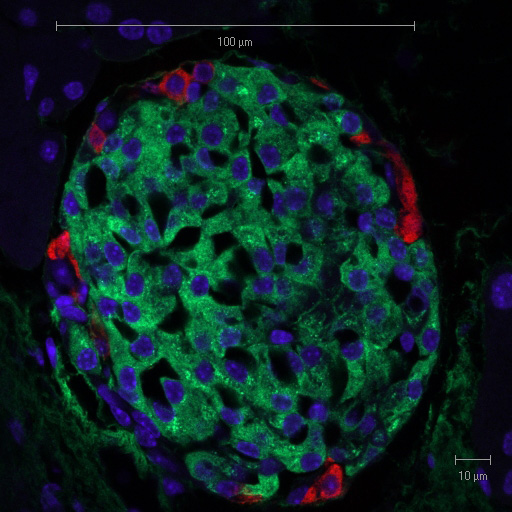
\includegraphics[width=0.9\textwidth]{billeder/forside.jpg}

\textsc{\center Bachelorprojekt \\
Projektnr: 15137 \\
Ingeniørhøjskolen, Aarhus Universitet \\
Den 16. december 2015 \\ \vspace{1cm}
11242	Anders Toft Andersen \\
201270874	Anders Esager \\
Projektvejleder: Samuel Alberg Thrysøe \\}
\end{center}

\cleardoublepage												% Indsaetter tom side, saa naeste kapitel starter paa hoejre side (hvis noedvendigt)
%% Dette er et titelblad designet til videregående uddannelser på et universitet
% Filen kræver:
% Universitetets logo:  AU-logo-DK eller AU-logo-DK
% Synopsis: En fil ved navn synopsis.tex

% Udarbejdet af: Jesper Nørgaard (jesper@noergaard.eu) 10. april 2012

\phantomsection
\pdfbookmark[0]{Titelblad}{titelblad}
\thispagestyle{empty}

\begin{minipage}[t]{0.48\textwidth}
\vspace*{-8pt}			

\includegraphics[height=2.5cm]{billeder/AU-logo-DK}
\end{minipage}
\hfill
\begin{minipage}[t]{0.48\textwidth}
{\small 
\textbf{Studienævn for Aarhus School of Science}\\
Nordre Ringgade 1 \\
8000 Aarhus C \\
Tlf: 8715 0000 \\
http://www.au.dk}
\end{minipage}

\vspace*{1cm}

\begin{minipage}[t]{0.48\textwidth}
\textbf{Titel:} \\[5pt]\bigskip\hspace{2ex}
Energirenovering

\textbf{Projekt:} \\[5pt]\bigskip\hspace{2ex}
P1-projekt

\textbf{Projektperiode:} \\[5pt]\bigskip\hspace{2ex}
September 2014 - December 2014

\textbf{Projektgruppe:} \\[5pt]\bigskip\hspace{2ex}
B131	

\textbf{Deltagere:} \\[5pt]\hspace*{2ex}
Adam  G. Hansen \\\hspace*{2ex}
Berit Jørgensen \\\hspace*{2ex}
Christoffer Haning \\\hspace*{2ex}
Dorthe Møller \\\hspace*{2ex}
Ejnar V. Jensen \\\hspace*{2ex}
Freja Poulsen \\\bigskip\hspace{2ex}
Gerhard Pedersen

\textbf{Vejledere:} \\[5pt]\hspace*{2ex}
Carsten Henningsen \\\bigskip\hspace{2ex}
Lotte Dalgaard

\vspace*{1cm}

\textbf{Oplagstal: 10} \\
\textbf{Sidetal: 80} \\
\textbf{Appendiks: 3} \\ 
\textbf{Afsluttet 18-12-2014}

\end{minipage}
\hfill
\begin{minipage}[t]{0.483\textwidth}
Synopsis: \\[5pt]
\fbox{\parbox{7cm}{\bigskipSynopsis

\bigskip}}
\end{minipage}

\vfill

{\footnotesize\itshape Rapportens indhold er frit tilgængeligt, men offentliggørelse (med kildeangivelse) må kun ske efter aftale med forfatterne.}

% Rapportens indhold er frit tilgængeligt, men offentliggørelse (med kildeangivelse) må kun ske efter aftale med forfatterne.
% The content of the report is freely available, but publication (with source reference) may only take place in agreement with the authors.

%\cleardoublepage
\chapter*{Forord}

Denne rapport er udarbejdet som en del af syvende semesters bachelorprojekt på Ingeniørhøjskolen, Aarhus Universitet. Rapporten er udarbejdet af en projektgruppe bestående af 2 sundhedsteknologistuderende. Projektet er udarbejdet i samarbejde med Søren Gregersen, overlæge på Medicinsk Endokrinologisk Afdeling på Aarhus Universitetshospital med hjælp fra Per. B. Jeppesen, Lektor ved Institut for Klinisk Medicin, Aarhus Universitet. Bachelorprojektet er udført i perioden 28. august 2015 til 16. december 2015, hvor forprojektet er udført i perioden 26. april 2015 til 15. juni 2015.  

Projektgruppen retter en stor tak til Søren Gregersen for samarbejdet, ligeledes skal der gives en tak til Per B. Jeppesen. Ydermere skal der lyde en varm tak til gruppens vejleder Samuel Thrysøe, der har hjulpet og støttet gruppen igennem hele processen. Endelig skal der gives en tak til reviewgruppen bestående af Simon Vammen Grønbæk og Karl-John Schmidt, som har bestået med konstruktiv kritik og rettelser. 


%Dette dokument indeholder projektdokumentationen for projektet \textit{Cell sorter for isolation of insulin producing cells}. Dokumentet indeholder kravspecifikation og accepttest for systemet, samt beskrivelse af projektets design og implementeringsfase. 

%Kravspecifikationen er udarbejdet i samarbejde med Søren Gregersen, overlæge på Medicinsk Endokrinologisk Afdeling, Aarhus Universitetshospital, der agerer som projektets kunde. 



\phantom{Luft}

\phantom{Luft}

\begin{table}[H]
	\centering
		\begin{tabular}{c c}
			\underline{\phantom{mmmmmmmmmmmmmm}} & \underline{\phantom{mmmmmmmmmmmmmm}}  \\
			Anders Toft Andersen			& Anders Esager		 			\\ 										\end{tabular}
\end{table}

\section*{Læsevejledning}
Rapporten indeholder primært metoder, resultater og diskussioner til produktet, som gruppen har udarbejdet. Der vil igennem rapporten fremtræde kildehenvisninger, og disse vil være samlet i en kildeliste bagerst i rapporten. Der er i rapporten anvendt kildehenvisning efter Harvardmetoden, i teksten refereres en kilde med [Efternavn, År]. Denne henvisning fører til kildelisten, hvor bøger er angivet med forfatter, titel, udgave og forlag, mens internetsider er angivet med forfatter, titel og dato. Til sidst i rapporten er bilagsliste, som anskueliggør filnavnene i den afleverede bilagsmappen. Diagrammerne udarbejdet i projektet er skrevet på engelsk. 

I bilagslisten forefindes alle filerne, der er afleveret ved siden af rapporten, herunder datablade, Matlab-kode, Eagle kilde-filer og Gerber-filer. Herudover er den udfyldte accepttest og fejlrapport vedlagt som bilag.

Ved siden af rapporten er vedlagt en video, som viser den udviklede prototype.

%Der vil igennem rapporten fremtræde kildehenvisninger, og disse vil være samlet i en kildeliste bagerst i rapporten. Der er i rapporten anvendt kildehenvisning efter Harvardmetoden, så i teksten refereres en kilde med [Efternavn, År]. Denne henvisning fører til kildelisten, hvor bøger er angivet med forfatter, titel, udgave og forlag, mens Internetsider er angivet med forfatter, titel og dato. Figurer og tabeller er nummereret i henhold til kapitel, dvs. den første figur i kapitel 7 har nummer 7.1, den anden, nummer 7.2 osv. Forklarende tekst til figurer og tabeller findes under de givne figurer og tabeller.

%\cleardoublepage

%%%% Indholdsfortegnelse (TOC) %%%%

\phantomsection													% Kunstigt afsnit, som hyperlinks kan 'holde fast i'
\pdfbookmark[0]{Indholdsfortegnelse}{indhold}					% Tildeler en klikbar bookmark til den endelige PDF
\tableofcontents*												% Indholdsfortegnelsen (kaldet ToC) 

%\addtocontents{toc}{\protect\newpage}							% Fremtvinger sideskift i ToC hvis noedvendig (der hvor koden placeres)


\mainmatter														% Hovedindhold - nummereres fra side 1

%%%% Rapportindhold %%%% 										% Rapportindholdet boer IKKE indeholde broedtekst - KUN includede filer!

%% Indledende %%												% Opdel evt. i passende afsnit for overblikkets skyld

%\section{Indledning}
Dette dokument indeholder accepttesten for the Cell Collector(omtales herefter som systemet). 

\subsection{Formål}
Formålet med dokumentet er at sikre at alle krav til produktet er opfyldt, i henhold til kravspecifikationen.

%\chapter{Projektbeskrivelse}

Projektforslaget lægger op til at belyse effekterne af energirenovering samt hvordan barrierne overvindes ved brug af virkemidler. 

I det følgende reflekteres der over emnerne i problemanalysen. Problemformuleringen indrammer herefter projektet inden det konkretiseres i afgrænsningen. Endelig beskrives de metoder, som søges anvendt. 

\section{Problemanalyse}

\section{Problemformulering}

I den kontekstuelle del søges følgende spørgsmål besvaret.

I den tekniske del søges følgende energi- og konstruktionsmæssige spørgsmål besvaret.

\section{Projektafgrænsning}

\section{Metode}
\section*{Resume}
\textbf{Baggrund}
Insulin er et essensielt hormon til regulering af glukose i blodet. Et fald i insulin produktionen ved nedsat funktion i de langerhanske øer kan føre til den livstruende sygdom \textit{diabetes mellitus}. Til at undersøge sygdommen og funktionen af de insulin producerende øer laves der videnskabelige forsøg med langerhanske øer fra mus. Denne proces foregår ved operativt at fjerne pankreas for herefter at opløse den ved hjælp af enzymet \textit{collagenase}. De enkelte øer isoleres herefter ved manuelt, at plukke dem fra en petriskål. Denne proces er både besværlig og tidskrævende. Derfor ønskes der nye metoder til isolering af langerhanske øer.

\textbf{Metoder} I gennem en agil udviklingsproces er der udviklet en \textit{Proof of Concept} prototype til automatisk isolering af langerhanske øer. Udviklingsfasen bestod af overordnede af fem faser, hhv. koncept fase, kravspecifikation, design, implementering og accepttest. Projektets overordnede tidsplan er opbygget som en stage gate model, hvor de enkelte udviklingsfaser er fastlagt med deadlines. I samarbejde med projektets review gruppe er de enkelte faser reviewed efter endt deadline. For at holde styr på arbejdsopgaverne er scrum værktøjet PivotalTracker anvendt, som har givet et overblik over de enkelte ugers sprints.

\textbf{Resultater og diskussion} Den udviklede prototype består af et software program udviklet i \textit{Matlab}, samt en række hardware komponenter. Prototypen virker vha. af billedprocessering, som detekterer de enkelte øer når de passerer et kamera. Ved detektion isoleres øen vha. en ventil i en seperat beholder. En enhedstest af det indkøbte kamera viste, at det ikke var tilstrækkelig kvalitet til detektering af øerne. Derfor er der i prototypen implementeret en funktion til simulering af kameraet ud fra genererede billeder.
  
Herudover er en cost-benefit analyse udarbejdet til at belyse, hvilke økonomiske fordele en automatiseret løsning vil have.   
%Projektet har yderligere givet et indblik i hvilke problemstillinger der skal løses inden en fungerende prototype kan implementeres i praksis, herunder hvorvidt øerne tager skade af processen. 


\textbf{Konklusion} Projektet har vist, at det er muligt at detektere langerhanske øer vha. billedprocessering ud fra genererede billeder. Systemet har desuden vist sig, at være velegnet til isolering af objekterne i simuleringsvæsken. Projektet har yderligere givet et indblik i hvilke problemstillinger der skal løses inden en fungerende prototype kan implementeres i praksis, herunder hvorvidt øerne tager skade af processen. 

Resultatet af cost-benefit analysen giver incitament til, at arbejde videre med en automatiseret løsning til isolering af øerne. 


\section*{Abstract}
\textbf{Background}

\blindtext

\textbf{Methods}

\blindtext

\textbf{Results}

\blindtext

\textbf{Discussion}


\textbf{Conclusion}


\chapter{Indledning}
Insulin er et essentielt hormon til regulering af glukose i blodet. Produktionen af insulin foregår i pancreas, nærmere bestemt i de Langerhanske øer. Et fald i insulin produktionen grundet nedsat funktion af de Langerhanske øer kan medføre den livstruende sygdom \textit{diabetes mellitus (type 1)}. Prævalensen af diabetes mellitus er i Danmark på 320.545, hvor omkring 10 \% lider af type 1 diabetes. \fxnote{Ref til: http://www.diabetes.dk/presse/diabetes-i-tal/diabetes-i-danmark.aspx}




\section*{Læsevejledning}
Skal nok flyttes op i forord

\section{Baggrund}
For at undersøge sygdommen nærmere, samt øge forståelsen for de mekanismer, der styrer insulinreguleringen i kroppen udføres der videnskabelige forsøg med Langerhanske øer.

De øer der anvendes til videnskabelige forsøg stammer typisk fra mus eller rotter. Sortering- og isoleringsprocessen foregår ved tre faser \citep{per}, som vist i figur \ref{fig:sortproces}. 

\begin{figure}[H]
	\centering
	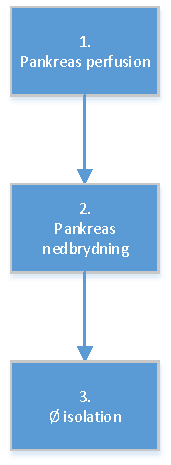
\includegraphics[width=0.2\textwidth]{billeder/sortering-crop.pdf}
	\caption{Faser i sorteringsprocessen}
	\label{fig:sortproces}
\end{figure}

I første fase, \textit{pankreas perfusion}, sprøjtes enzymet \textit{collagenase V} ind gennem galdegangene og derfra videre til  pankreas. Dette enzym starter en nedbrydning af vævet i pankreas. Herefter fjernes pankreas operativt. Enzymet collagenase har den egenskab, at det ikke nedbryder de langerhanske øer i samme grad som det omkringliggende eksokrine væv.

I anden fase, \textit{pankreas nedbrydning}, nedbrydes pankreas yderligere ved at inkubere pankreas ved 37° i 19 min. Ved denne temperatur er enzymet collagenase særligt aktivt og katalysere derfor nedbrydningen af pankreas. Herefter nedkøles vævet for at stoppe virkningen af collagenase.

% sker derfor relativt hurtigt.  den bliver skåret i mindre dele og pankreas placeres i en inkubator ved 37,5 grader. Dette gøres for at accelerere nedbrydningen af pankreas. Når pankreas er nedbrudt nedkøles vævet for, at stoppe virkningen af collagenase. 

I den sidste fase, \textit{ø isolation}, vaskes og rystes øerne først af tre omgange med en vaskebuffer i form af en saltvandsopløsning \citep{hbbs}. Dette gøres for at løsrive øerne fra hinanden inden isolering. Herefter er øerne klar til at blive isoleret fra det eksokrine væv. Der findes en række forskellige metoder til dette, hvor den mest udbredte metode foregår ved manuel isolering af øerne fra en petriskål vha. et mikroskop. Der bruges allerede automatiserede isoleringsmetoder bygget på forskellige teknikker, herunder gradientbaseret centrifugering. Fælles for de anvendte teknikker til isolering af øerne er, at der er stor risiko for skade på øerne. 

Denne manuelle metode har yderligere ulemper, idet den både er besværlig og tidskrævende. Herudover kan der være stor variation i kvaliteten af isoleringen, da der kan være forskel på den enkelte operatørs håndtering af øerne. 

Derfor ønskes der en automatiseret metode til isolering af langerhanske øer, med minimal risiko for skader på øerne. En automatiseret metode vil have følgende fordele \cite{pptintro}: 

\begin{itemize}
\item Øget sorteringshastighed for højere udbytte
\item Reducere variation i de isolerede øer
\item Reducere omkostningerne
\item Sikre bedre dokumentation
\item Forbedret arbejdsmiljø
\end{itemize} 

En automatiseret løsning vil potentielt åbne op for nye muligheder indenfor anvendelse af langerhanske øer. Der forskes bl.a. i transplantation af langerhanske øer, som et led i behandling af type 1 diabetes. Resultaterne af et af disse forskningsprojekter har bl.a. vist at 44 \% af modtagerne af denne type behandling var insulinuafhængige 3 år efter transplantation \citep{islettransplantation}. Til forskning er langerhanske øer bl.a. anvendt til at undersøge hvordan aminosyrer er glukoseafhængige \citep{aminosyre}. I forskningsforsøget er der brugt 6-10 mus, hvilket cirka har taget 6-10 timer at håndplukke (jvf. Per B. Jeppesen). Det er forskningsprojekter som dette, hvor en automatiseret løsning vil være relevant, da det vil skabe en mulighed for en større testgruppe og frigive ressourcer til andre formål i forsøget.

\newpage
På Medicinsk Endokrinologisk Afdeling (MEA), Aarhus Universitetshospital, er der tidligere arbejdet hen imod en automatiseret løsning til isolering af langerhanske øer. Den automatiseret løsning vil primært bidrage til forskningen, der foretages på afdelingen. Tidligere blev der udviklet en prototype til automatiseret ø-isolation, der fungerede ved hjælp af kameradetektion. Ved detektion sugede en pipette den detekterede ø op fra en petriskål. Pipetten blev styret i X,Y og Z retning vha. en mekanisk robotarm. Se figur \ref{fig:Tidliger prototype} for en illustration af den gamle prototype. \footnote{Kilde: Søren Gregersen}

\begin{figure}[H]
	\centering
	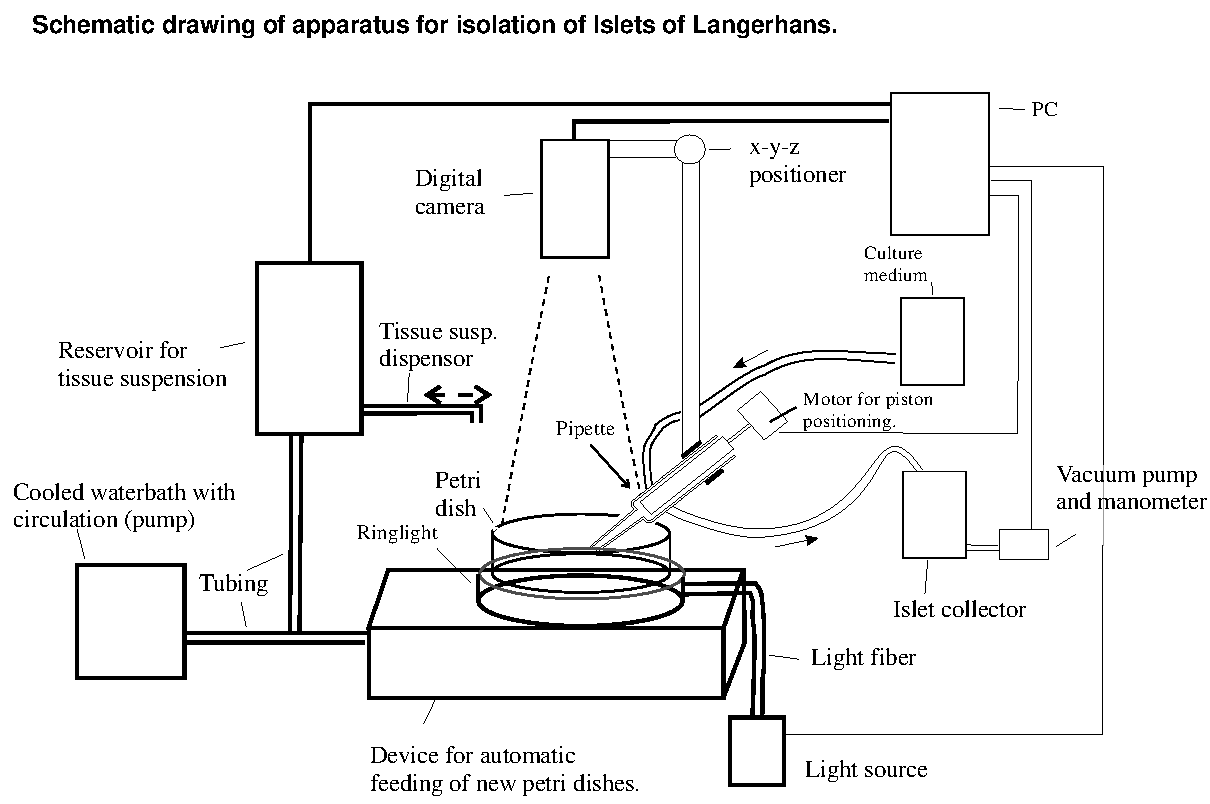
\includegraphics[width=1\textwidth]{billeder/hovedrapport/glprototype.pdf}
	\caption{Tidligere prototype}
	\label{fig:Tidliger prototype}
\end{figure}


 Prototypen var dog ikke præcis nok, primært pga. bevægelse i væsken, og projektet blev derfor stoppet.
 

%\textbf{Noter:}
%
%kilder om transplantation af øer
%
%
% 
% 
% find videnskabelige artikler der bekræfter at denne metode med at skyde langerhanske øer ind i sukkersyge mus/rotter virker og det er derfor dette projekt er mega relevant og pisse godt
% 
% derfor
% 
% - videnskabelig artikel over sorteringsprocessen
% 
% - videnskabelig artikel over at metoden virker, evt. hvorfor den ikke er mere brugt(sorteringsprocessen er for langsommelig)





\section{Problemformulering}
Formålet med projektet er, at udvikle et \textit{Proof of Concept} system til isolering af langerhanske øer baseret på .... metoden.

Det udviklede system skal kunne detektere langerhanske øer vha. billedprocessering. Ved detektion skal øerne isoleres fra opløsningen. 

Herudover skal en cost-benefit analyse være med til at belyse hvilke økonomiske og kvalitative fordele det udviklede system vil have i sorteringsprocessen.

\section{Afgrænsning}
Til at afgrænse projektet anvendes \textbf{M}o\textbf{SC}o\textbf{W} modellen, som beskriver hvilke dele projektet skal (\textbf{M}ust), bør (\textbf{S}houd), kan (\textbf{C}ould og ikke (\textbf{W}ont) indeholde. MoSCoW modellen (figur: \ref{fig:moscow}) viser hvordan de enkelte krav og dele af projektet er prioriteret. 
Redegørelse og begrundelser for valg/fravalg
Moscow

\begin{figure}[H]
	\centering
	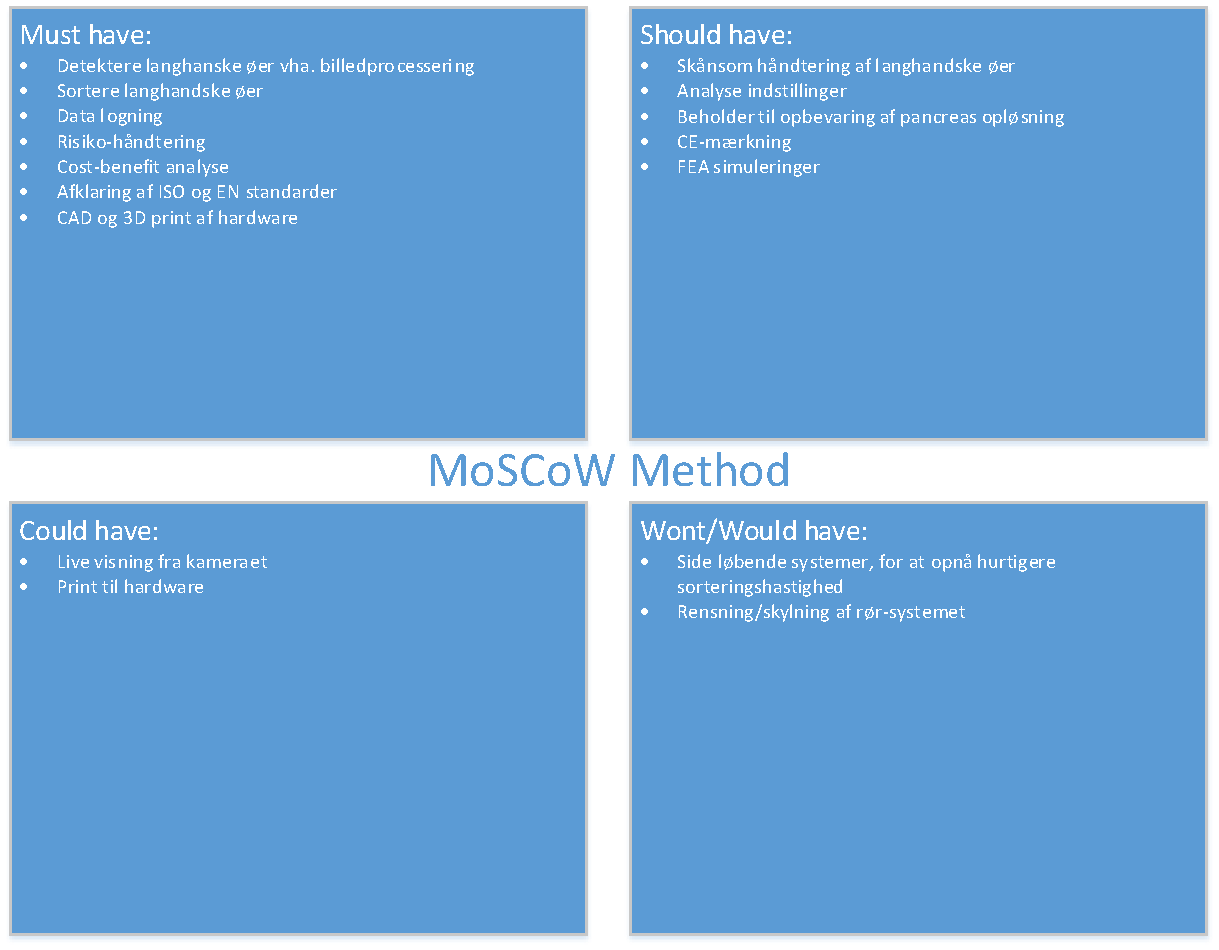
\includegraphics[width=1\textwidth]{billeder/MoSCoW-crop.pdf}
	\caption{MoSCoW}
	\label{fig:moscow}
\end{figure}

De krav systemet skal opfylde er bl.a. at kunne detektere langerhanske øer vha. billedprocessering, samt sortere øerne ved detektion. Herudover skal systemet kunne gemme data omkring de sorterede øer herunder størrelse og cirkularitet. Projektet består desuden af en cost-benefit analyse der beskriver hvilke fordele og ulemper det automatiserede system vil have. 

Et af de vigtigere krav der er nedprioteriet i projektet er skånsom håndtering af langerhanske øer. Denne del vil kræve en validering af den udviklede prototype igennem funktionstest af de isolerede langerhanske øer. Referencer til dette?

Dette projekt vil derfor i højere grad fokusere på en verificering af den udviklede prototype i form af en accepttest, som tester de funktionelle og ikke funktionelle krav.

\chapter{Systembeskrivelse}
Dette kapitel indeholder en introducerende beskrivelse af den udviklede prototype. Herudover indeholder kapitlet en beskrivelse af opløsningen med de langerhanske øer.

Figur \ref{fig:system} viser den overordnede opbygning af \textit{The Cell Collector}, benævnes herefter som systemet. Grundlæggende består systemet af en beholder, hvor i opløsningen med langerhanske øer er. Opløsningen pumpes herefter ved hjælp af en pumpe i gennem en slange, hvor et kamera detekterer om en ø passerer eller ej. Hvis en ø detekteres åbner systemet en ventil for at frasortere øen fra resten af opløsningen. Systemet består af et software program udviklet i \textit{Matlab}, hvor operatøren har mulighed for at interagere med systemet. Her er selve logikken og signalbehandlingen i form af billedprocessering implementeret. Programmet giver signal til en microcontroller (Arduino platform), som håndterer den videre styring af hardwarekomponenterne.

\begin{figure}[H]
	\centering
	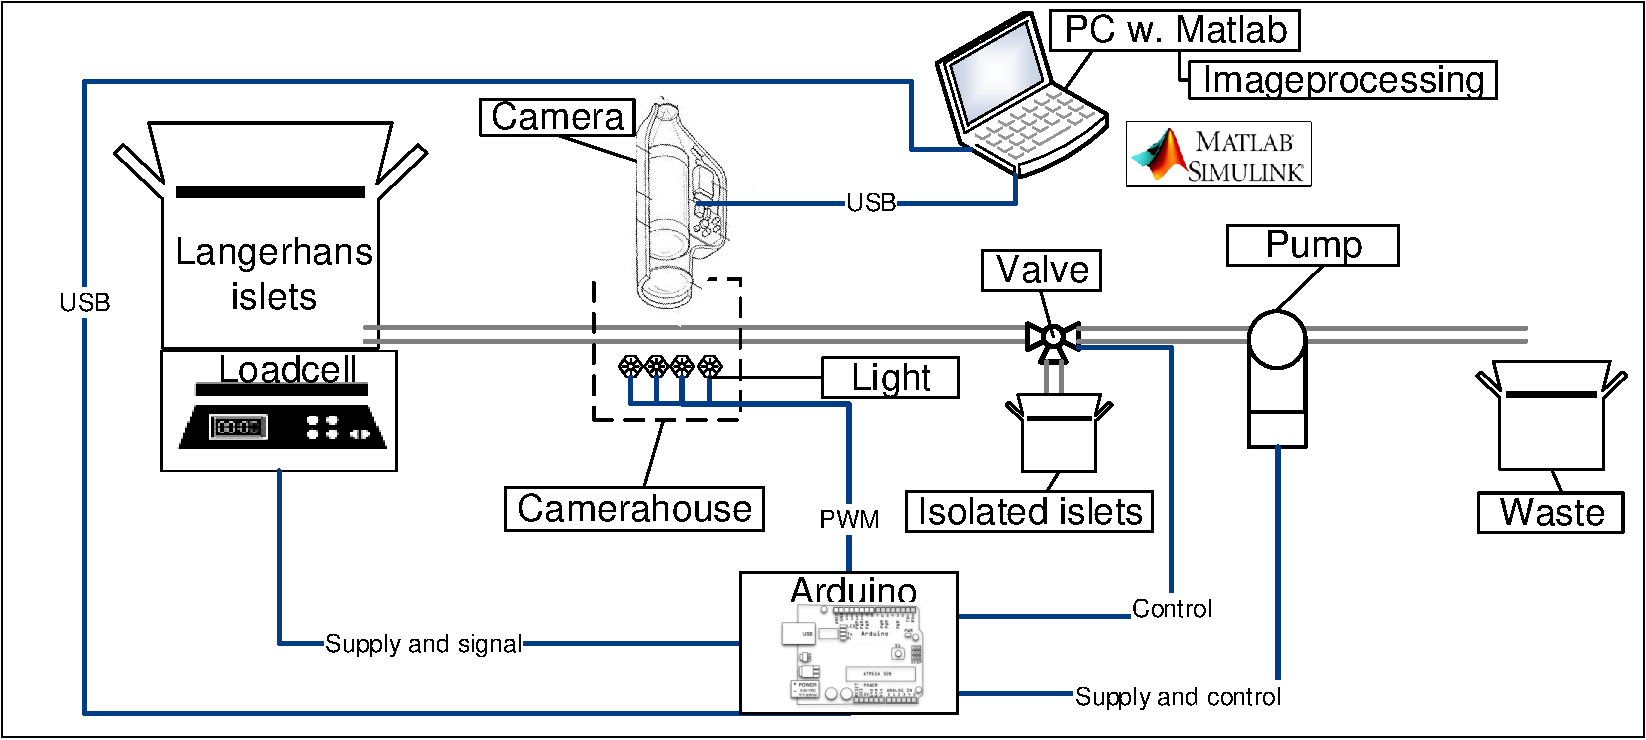
\includegraphics[width=1\textwidth]{billeder/DMTS.pdf}
	\caption{Figuren viser den overordnede opbygning af systemet}
	\label{fig:system}
\end{figure}
%Beskrivelse 
%
%Figur over systemet
%
%Billeder af det færdige system


%\section{Sorteringsproces}
%Dette afsnit beskriver hvordan sorteringsprocessen foregår, samt generelle egenskaber for opløsningen med langerhanske øer. 
%
%\subsection{Sorteringsproces} \label{subsec:sortproces} \fxnote{Vi venter stadig på den faktiske protokol fra SG}
%Som det kort blev beskrevet i baggrundsafsnittet består isoleringen af langerhanske øer af 3 faser. 
%Figur \ref{fig:sortproces} viser den trinvise proces fra intakt pankreas til isoleret ø.
%
%\begin{figure}[H]
%	\centering
%	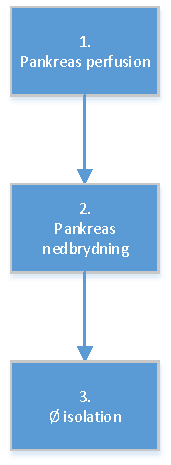
\includegraphics[width=0.2\textwidth]{billeder/sortering-crop.pdf}
%	\caption{Sorteringsproces}
%	\label{fig:sortproces}
%\end{figure}
%
%Den første fase, \textit{pankreas perfusionen}, foregår ved at man først operativt fjerner pancreas, hvorefter enzymet collagenase sprøjtes ind i pankreas. Dette enzym starter en nedbrydning af vævet i pankreas. Enzymet har den egenskab, at det ikke nedbryder de langerhanske øer, men derimod kun det omkringliggende væv.
%
%I anden fase, \textit{pankreas nedbrydningen}, nedbrydes pankreasen yderligere ved at den bliver skåret i mindre dele og pankreas placeres i en inkubator ved 37,5 grader. Dette gøres for at accelerere nedbrydningen af pankreas. Når pankreas er nedbrudt nedkøles vævet for, at stoppe virkningen af collagenase. 
%
%I den sidste fase, \textit{ø isolation}, bliver øerne frasorteret fra det omkringliggende væv. 

\newpage
\section{Langerhanske øer}
Dette afsnit beskriver nærmere opløsningen med de langerhanske øer. Den endelige opløsning består udover øerne af eksokrint væv fra pankreas, samt af en saltvandopløsning (\cite{hbbs}). 

Figur \ref{fig:islet} viser hvordan opløsningen ser ud, når den er hældt i en petriskål. På billedet er øerne markeret med en rød cirkel.

\begin{figure}[H]
	\centering
	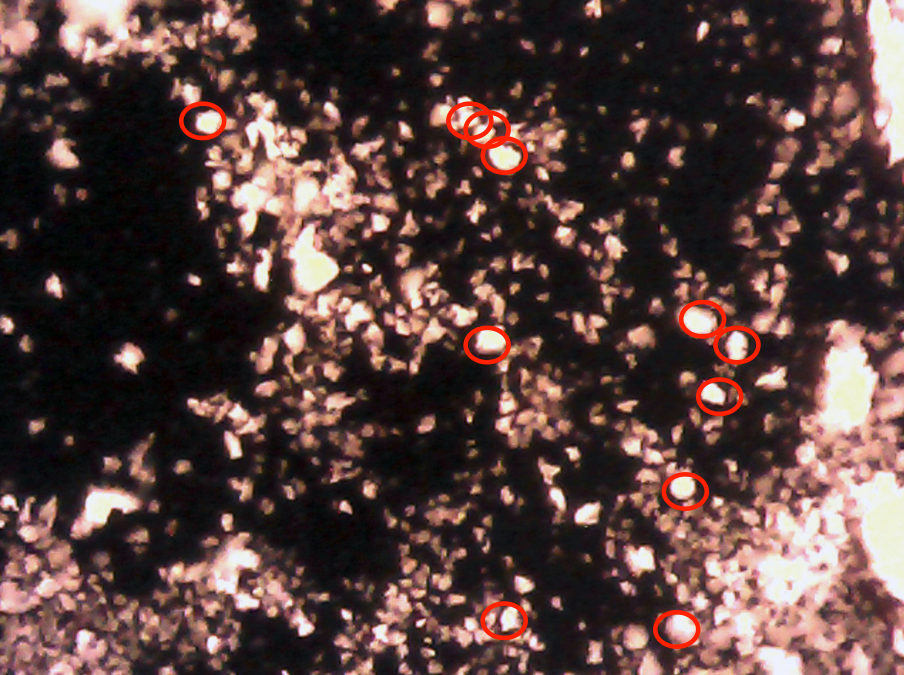
\includegraphics[width=0.5\textwidth]{billeder/software/sgbillede.png}
	\caption{Opløsning med langerhanske øer. Øerne er markeret med en rød cirkel}
	\label{fig:islet}
\end{figure}

Et batch af langerhanske øer, som opnåes ved en typisk sorteringsproces på Medicinsk Endokrinologisk Afdeling består af mellem 300 og 400 øer. For at få et udbytte på 300 til 400 øer anvendes typisk mellem 5 og 6 mus. Den samlede mængde opløsningsvæske for sådan et batch er omkring 150 ml.

De generelle fysiske egenskaber for de langerhanske øer er en størrelse mellem 100 og 300 um, samt at de er forholdsvis runde. Herudover har de en højere lysintensitet end det eksokrine væv. Det vil bl.a. være disse parametre kameraet skal detektere øerne på.






%\section{Baggrund}
For at undersøge sygdommen nærmere, samt øge forståelsen for de mekanismer, der styrer insulinreguleringen i kroppen udføres der videnskabelige forsøg med Langerhanske øer.

De øer der anvendes til videnskabelige forsøg stammer typisk fra mus eller rotter. Sortering- og isoleringsprocessen foregår ved tre faser \citep{per}, som vist i figur \ref{fig:sortproces}. 

\begin{figure}[H]
	\centering
	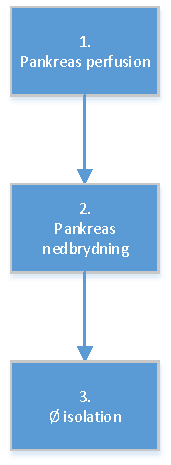
\includegraphics[width=0.2\textwidth]{billeder/sortering-crop.pdf}
	\caption{Faser i sorteringsprocessen}
	\label{fig:sortproces}
\end{figure}

I første fase, \textit{pankreas perfusion}, sprøjtes enzymet \textit{collagenase V} ind gennem galdegangene og derfra videre til  pankreas. Dette enzym starter en nedbrydning af vævet i pankreas. Herefter fjernes pankreas operativt. Enzymet collagenase har den egenskab, at det ikke nedbryder de langerhanske øer i samme grad som det omkringliggende eksokrine væv.

I anden fase, \textit{pankreas nedbrydning}, nedbrydes pankreas yderligere ved at inkubere pankreas ved 37° i 19 min. Ved denne temperatur er enzymet collagenase særligt aktivt og katalysere derfor nedbrydningen af pankreas. Herefter nedkøles vævet for at stoppe virkningen af collagenase.

% sker derfor relativt hurtigt.  den bliver skåret i mindre dele og pankreas placeres i en inkubator ved 37,5 grader. Dette gøres for at accelerere nedbrydningen af pankreas. Når pankreas er nedbrudt nedkøles vævet for, at stoppe virkningen af collagenase. 

I den sidste fase, \textit{ø isolation}, vaskes og rystes øerne først af tre omgange med en vaskebuffer i form af en saltvandsopløsning \citep{hbbs}. Dette gøres for at løsrive øerne fra hinanden inden isolering. Herefter er øerne klar til at blive isoleret fra det eksokrine væv. Der findes en række forskellige metoder til dette, hvor den mest udbredte metode foregår ved manuel isolering af øerne fra en petriskål vha. et mikroskop. Der bruges allerede automatiserede isoleringsmetoder bygget på forskellige teknikker, herunder gradientbaseret centrifugering. Fælles for de anvendte teknikker til isolering af øerne er, at der er stor risiko for skade på øerne. 

Denne manuelle metode har yderligere ulemper, idet den både er besværlig og tidskrævende. Herudover kan der være stor variation i kvaliteten af isoleringen, da der kan være forskel på den enkelte operatørs håndtering af øerne. 

Derfor ønskes der en automatiseret metode til isolering af langerhanske øer, med minimal risiko for skader på øerne. En automatiseret metode vil have følgende fordele \cite{pptintro}: 

\begin{itemize}
\item Øget sorteringshastighed for højere udbytte
\item Reducere variation i de isolerede øer
\item Reducere omkostningerne
\item Sikre bedre dokumentation
\item Forbedret arbejdsmiljø
\end{itemize} 

En automatiseret løsning vil potentielt åbne op for nye muligheder indenfor anvendelse af langerhanske øer. Der forskes bl.a. i transplantation af langerhanske øer, som et led i behandling af type 1 diabetes. Resultaterne af et af disse forskningsprojekter har bl.a. vist at 44 \% af modtagerne af denne type behandling var insulinuafhængige 3 år efter transplantation \citep{islettransplantation}. Til forskning er langerhanske øer bl.a. anvendt til at undersøge hvordan aminosyrer er glukoseafhængige \citep{aminosyre}. I forskningsforsøget er der brugt 6-10 mus, hvilket cirka har taget 6-10 timer at håndplukke (jvf. Per B. Jeppesen). Det er forskningsprojekter som dette, hvor en automatiseret løsning vil være relevant, da det vil skabe en mulighed for en større testgruppe og frigive ressourcer til andre formål i forsøget.

\newpage
På Medicinsk Endokrinologisk Afdeling (MEA), Aarhus Universitetshospital, er der tidligere arbejdet hen imod en automatiseret løsning til isolering af langerhanske øer. Den automatiseret løsning vil primært bidrage til forskningen, der foretages på afdelingen. Tidligere blev der udviklet en prototype til automatiseret ø-isolation, der fungerede ved hjælp af kameradetektion. Ved detektion sugede en pipette den detekterede ø op fra en petriskål. Pipetten blev styret i X,Y og Z retning vha. en mekanisk robotarm. Se figur \ref{fig:Tidliger prototype} for en illustration af den gamle prototype. \footnote{Kilde: Søren Gregersen}

\begin{figure}[H]
	\centering
	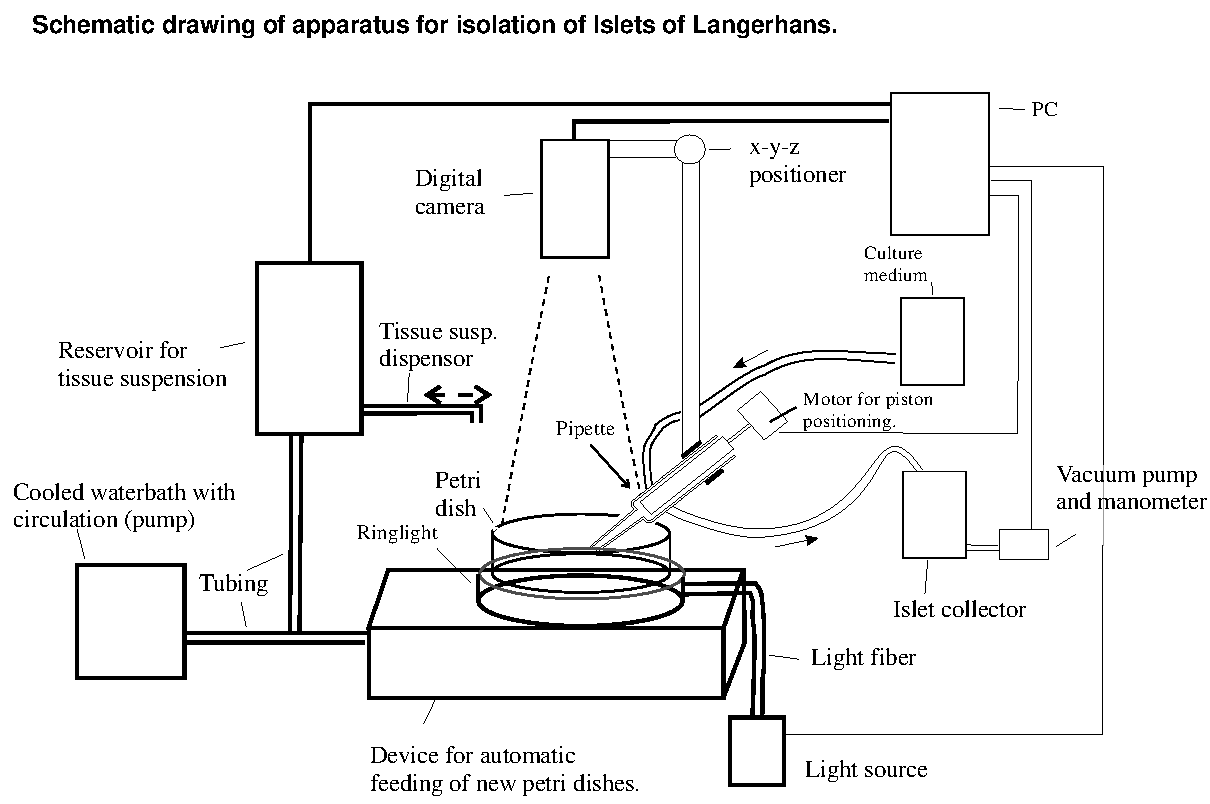
\includegraphics[width=1\textwidth]{billeder/hovedrapport/glprototype.pdf}
	\caption{Tidligere prototype}
	\label{fig:Tidliger prototype}
\end{figure}


 Prototypen var dog ikke præcis nok, primært pga. bevægelse i væsken, og projektet blev derfor stoppet.
 

%\textbf{Noter:}
%
%kilder om transplantation af øer
%
%
% 
% 
% find videnskabelige artikler der bekræfter at denne metode med at skyde langerhanske øer ind i sukkersyge mus/rotter virker og det er derfor dette projekt er mega relevant og pisse godt
% 
% derfor
% 
% - videnskabelig artikel over sorteringsprocessen
% 
% - videnskabelig artikel over at metoden virker, evt. hvorfor den ikke er mere brugt(sorteringsprocessen er for langsommelig)



\chapter{Metoder}
Dette kapitel indeholder beskrivelser af hvordan projektet er udført, og hvilke metoder, der er brugt. Yderligere indeholder kapitlet projektstyring, samt hvilke modeller, der er fulgt igennem projektforløbet. 

\section{Samarbejdsaftale}
For at sikre gruppens enighed i udførelse af projektet, om bla. arbejdsindsats samt timer der skulle bruges på projektet, blev der udarbejdet en samarbejdsaftale. Samarbejdsaftalen bevirker derfor som en forventningsafstemning. Se samarbejdsaftalen i bilag \ref{bilag:samarbejdsaftale}

\section{Samarbejdspartnere}
Gruppens kunde er Søren Gregersen, overlæge på Medicinsk Endokrinologisk Afdeling, Aarhus Universitetshospital. Det er i samarbejde med Søren, at projektet er blevet specificeret, samt hvilke krav der er til den endelige prototype.
Samuel Alberg Thrysøe er gruppens projektvejleder. Der er afholdt ugentlige vejledermøder, hvor gruppen har givet status på projektet og hvor der er diskuteret forskellige problemstillinger. Til hvert vejledermøde har der været en dagsorden med punkter, som formål og begrundelse for punkterne på dagsorden. Dagsordenerne er sendt til vejleder senest en dag før vejledermødet. Dette er gjort for at give vejleder en chance for at forberede sig på den givne dagsorden. Til hvert vejledermøde er der udført et referat som kan ses i bilag \ref{modevejleder}.
Simon Vammen Grønbæk og Karl-Johan Schmidt har fungeret som projektets reviewgruppe. Der er holdt møde hver tredje uge omhandlende aftalt dagsorden. Formålet med reviewgruppen er, at få konstruktiv feedback på evt. rettelser, opbygning af rapport og generel forståelse. Reviewgruppen har været gode til at sparre med omkring diskussioner, samt andre spørgsmål i gruppen. Dette har været med til at drive projektet igennem udviklingsfaserne, da deadlines har været fastlagt i samarbejdet med reviewgruppen.

Reviewmøderne har forgået ved, at grupperne har udvekslet dokumenterne, der skulle reviews. Grupperne har skrevet kommentar til dokumentet, hvorefter kommentarene og rettelserne er diskuteret på møderne. 

\newpage
\section{Udviklingsværktøjer}
Dette afsnit består af en kort beskrivelse omkring udviklingsværktøjer brugt i projektet.

\textbf{MATLAB:} Softwaren til systemet er udviklet i \textit{MATLAB}. Versionen, der er anvendt, er R2015b. Tilføjelsespakker brugt i projektet er følgende:
\begin{itemize}
\item Arduino Support Package (14.2.2)
\item Webcam Support Package (15.2)
\end{itemize}
Disse pakker anvendes til at interagere med Arduinoen og USB mikroskopet. 

\textbf{Fritzing:} \textit{Fritzing} er brugt til at illustrere kredsløbsdiagrammer(schematics), samt enhedstest af hardwaren ved illustrationer af \textit{fumlebræt}. Dette har bidraget til dokumentationen af  enhedstestene. Derudover har det givet mulighed for, at opstillingerne brugt på \textit{fumlebræt}, let kunne genskabes.

\textbf{Eagle:} \textit{Eagle} er et program til udarbejdelse af print layouts. \textit{Eagle} er brugt til at lave et samlet PCB layout for hardwareelementerne. I \textit{Eagle} er der generet Gerber-filer, som er sendt til PCB fabrikanten.

\textbf{SolidWorks:} \textit{SolidWorks} er et program til at illustrere mekaniske 3D modeller med.  \textit{SolidWorks} er brugt til at lave kamerahuset med for senere, at få det 3D printet.

\textbf{Arduino IDE:} Programmet som er udbudt af \textit{Arduino} bruges til at programmere \textit{Arduino} udviklingskortet. \textit{Arduino IDE} er i projektet brugt til enhedstest for at teste hardware opstillingerne. 

\textbf{Microsoft Visio:} \textit{Microsoft Visio} er et tegne program, som bruges til at illustrere forskellige modeller. Programmet er valgt til at lave udviklingsdiagrammer og illustrationer med. 

\textbf{Texmaker:} Dette program er brugt til at skrive alt dokumentationen i projektet. \textit{Texmaker} gør det muligt at arbejde på samme dokument samtidigt, hvilket har været en stor hjælp.

\textbf{PivotalTracker:} \textit{PivotalTracker} er et scrumbaseret projektstyringsværktøj, der hjælper med at styre arbejdsressourcerne i projektet. Der er i afsnittet \ref{subsec:agil} uddybet hvordan \textit{PivotalTracker} er brugt i projektet.

\textbf{GitHub:} Er et versionsstyringsprogram, som i projektet er brugt til versionsstyring af dokumenter og \textit{Matlab} koden til projektet. Se afsnit \ref{subsec:github} for uddybende dokumentation omkring hvordan \textit{Github} er benyttet.

\textbf{Dropbox:} Det cloudbaserede delingsværktøj \textit{Dropbox} er i projektet brugt til at gemme og dele artikler, diagrammer, billeder og generelle noter.

\textbf{Microsoft Onenote:} \textit{Onenote} er et program til at lave noter i. I projektet er programmet brugt til at have fælles noter og huskelister.


\newpage
\section{Versionsstyring}
I projektet er der gjort brug af versionsstyringssoftwaren \textit{GitHub}. Til store ændringer har dokumenterne fået et nyt versionsnummer og versionshistorikstabellen er opdateret i hvert dokument, se tabellen nedenfor. 

\begin{center}
		\begin{longtable}{ | m{1.5cm} | m{2cm}| m{7cm}| m{2cm}| } 
			\hline
			\textbf{Version}  & \textbf{Dato} & \textbf{Beskrivelse} & \textbf{Initialer}  \\ 
			\hline
			0.1  &  19/09 2015  & Dokument sendt til review & AE og AT \\
			\hline
		1.0  &  19/09 2015  & Rettelser fra reviewmøde og Latex layout & AE og AT \\
		\hline
		1.1  &  20/10 2015  & Kamerakrav tilføjet & AE og AT \\
		\hline
		2.0  &  6/11 2015  & Definitioner og layout ændringer & AE og AT \\
			\hline
		\end{longtable}
		
	\end{center}


\subsection{Github}
\label{subsec:github}
Til versionsstyring af projektdokumentationen og source kode anvendes GitHub, som bygger på open source versionsstyringssystemet Git. Her opdateres der løbende ændringer, så det nyeste dokumentation og source kode altid er tilgængeligt. 
Som user interface til GitHub anvendes GitHub Desktop (figur: \ref{fig:git}). I GitHub Desktop vises en tidslinje, for hvornår, der er lavet ændringer. Under de enkelte filer kan det observeres, hvad der er ændret i for den gældende version. Programmet giver yderligere indblik, i hvilke filer, der lokalt er lavet ændringer i, som ikke er tilføjet repositoriet endnu.
\begin{figure}[H]
	\centering
	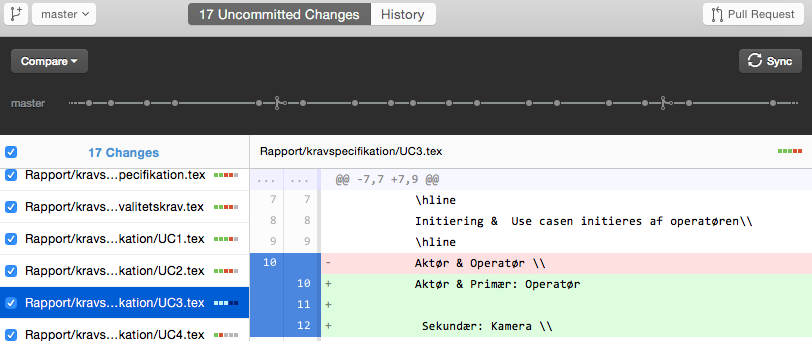
\includegraphics[width=1\textwidth]{billeder/github.png}
	\caption{GitHub Desktop}
	\label{fig:git}
\end{figure}
\newpage

\section{Projektstyring} 
Til projektstyring er der brugt en stage gate model. En stage gate model(figur \ref{fig:stage-gate}) er bestående af nogle udviklingsfaser(stages), hvor der er en deadline for de konkrete faser. For at komme til næste fase/stage, skal der være opfyldt nogle kriterier. Kriterierne opstilles i en tjekliste(se figur \ref{fig:stage-gate-tjekliste}), hvor de kan krydses af. Alle punkter skal være opfyldt for at komme igennem gaten. En stage gate model er god til at få et produkt på markedet, men det har sine svagheder ved en agil udviklingsprocess. Derfor er der i projektet arbejdet med åbne gates, hvilket gør det muligt at gå tilbage for at justere på dokumenter. I projektet er stage gate modellen brugt som tidsplan og en metode, der har været med til at sikre, at fasen var færdig inden næste fase igangsættes. 

%\begin{landscape}
\begin{figure}[H]
	\centering
	\includegraphics[width=0.65\textwidth]{billeder/Hovedrapport/Stage-gatel.PDF}
	\caption{Stage gate model}
	\label{fig:stage-gate}
\end{figure}
%\end{landscape}

\begin{figure}[H]
	\centering
	\includegraphics[width=0.7\textwidth]{billeder/Hovedrapport/Stagegatetjekliste.PDF}
	\caption{Stage gate tjekliste}
	\label{fig:stage-gate-tjekliste}
\end{figure}

%\begin{sidewaysfigure}
%\begin{figure}[H]
%	\centering
%	\includegraphics[width=0.6\textwidth]{billeder/Hovedrapport/Stage-gateP.PDF}
%	\caption{Stage gate model}
%	\label{fig:moscow}
%\end{figure}
%\end{sidewaysfigure}



%\begin{figure}
%  \begin{sideways}
%    \begin{minipage}{27.5cm}
%      \includegraphics[width=0.6\textwidth]{billeder/Hovedrapport/Stage-gateP.PDF}
%    \end{minipage}
%  \end{sideways}
%  \centering
%  \caption[Caption]{Caption.}
%  \label{pic:picture}
%\end{figure}

\subsection{Agil udviklingsproces}
\label{subsec:agil}
I projektet er der brugt en agil arbejdsproces hvor der konstant er fokus på at målrette og prioritere arbejdet, der giver mest værdi for projektet og kunden. Derfor er der løbende prioriteret mellem opgaverne, hvorefter delopgaverne er blevet revurderet og planlagt. Dette gør at produktet og resultater evalueres og testes løbende, hvilket danner grundlag for prioriteringen af opgaverne til næste periode(sprint). Til at sikre arbejdsressourcerne tilrådighed for projektet er brugt på den mest effektive måde, er der valgt at bruge elementer fra SCRUM. SCRUM er en iterativ arbejdsmetode, hvor  der er iterationer(sprints), som i dette projekt har haft en periode på en uge. SCRUM er brugt i projektet vha. \textit{Pivotaltracker}. 

I Pivotaltracker defineres projektets arbejdsopgaver, hvorefter de tildeles point alt efter hvor stor arbejdsbyrden er. De enkelte opgaver prioriteres herefter i projektets backlog, hvor Pivotaltracker automatisk tilføjer opgaver til den igangværende sprint udfra den nuværende “velocity”. Et nyt sprint påbegyndes automatisk når en ny uge starter.

Det betyder, at der er fuldstændig styr på om projektet går for langsomt, eller om udviklingen af projektet er godt med. Dette kan holdes op imod den tidligere nævnte stage gate model.

Herudover giver Pivotaltracker mulighed for en komplet log over projektets udførte opgaver og afsluttede sprints. Her kan man se hvilke opgaver, der er udført i hvilken uge. I projektet anvendes dette som logbog for udførte arbejdsopgaver. Se logbøgerne fra \textit{Pivotaltracker} i bilag \ref{bilag:Logboger}.

En opgave kan have forskellige states, som definerer dens status. Når en opgave er afsluttet kan den afleveres til review, hvor den herefter enten kan godkendes eller afvises. Dette er særligt anvendeligt i projektets udviklingsfase, hvor en feature kan testes og godkendes af et andet projektmedlem. Figur \ref{fig:pt_sprints}  viser et overblik over tidligere sprints, hvor figur \ref{fig:pt_currentsprint} viser en igangværende sprint med godkendte, afsluttet og endnu ikke færdiggjorte opgaver.

\begin{figure}[htbp] \centering
\begin{minipage}[b]{0.48\textwidth} \centering
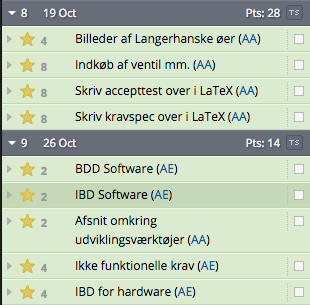
\includegraphics[width=1.00\textwidth]{billeder/pt_previous_sprints} % Left picture
\end{minipage} \hfill
\begin{minipage}[b]{0.48\textwidth} \centering
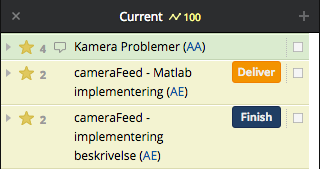
\includegraphics[width=1.00\textwidth]{billeder/pt_current_sprint} % Right picture
\end{minipage} \\ % Captions og labels
\begin{minipage}[t]{0.48\textwidth}
\caption{To færdiggjorte sprints} % Left caption and label
\label{fig:pt_sprints}
\end{minipage} \hfill
\begin{minipage}[t]{0.48\textwidth}
\caption{Igangværende sprint} % Right caption and label
\label{fig:pt_currentsprint}
\end{minipage}
\end{figure}

\section{Udviklingsfaserne}
Under udviklingen af projektet er der gennemgået fire faser. Den første fase i projektet har været konceptanalyse. Konceptanalysen bestod bl.a. af litteratursøgning omkring langerhanske øer, dette blev gjort for at opnå tilstrækkelig viden omkring størrelserne, deres egenskaber mm. Der blev søgt efter allerede eksisterende sorteringsmetoder, som blev anvendt på det daværende tidspunkt. Dette var primært for at opnå erfaring inden for området på kort tid. Efter litteratursøgningen blev et overordnet koncept etableret i samarbejde med kunden(\textit{Søren Gregersen}). Ydermere er det i konceptanalysen, at der er identificeret problemstillinger og afgrænsninger af projektet. Samtidigt med konceptanalysen, blev der fokuseret på produktionen af produktet. Det er gjort for at undgå løsninger, som ikke kan produceres eller er besværlige at fremstille. Til sidst i konceptfasen er der udarbejdet en tidsplan for projektet.

Den anden fase består af kravspecifikationen, hvilket er udarbejdet i tæt samarbejde med kunden. En kravspecifikation har sikret at kunde og projektudviklere er enige om projektets udformning. I kravspecifikationen er der brugt usecasediagram, samt fully dressed beskrivelser af hver usecase. Der laves fully dressed, for at klaregøre normal forløbet for hver usecase, samt undtagelser og udvidelser til dem. Derudover er det i kravspecifikationen, at der er specificeret ikke funktionelle krav og kvalitetskrav. Samtidigt med kravspecifikationen er der udarbejdet en accepttest. Denne test er med til at verificere at alle krav, der er bestemt i samarbejde med kunden, er opfyldte. I accepttesten er det beskrevet hvordan hver enkelt krav skal testes. Accepttesten udføres før produktet afleveres til kunden. Se afsnit \ref{subsec:krav} for eksempler.

Den tredje fase i projektet er designfasen, hvor der udfra kravspecifikationen er lavet overordnede diagrammer. Diagrammerne er brugt til at beskrive systemet og dele systemet op i mindre delsystemer. Det er diagrammerne, der er brugt til at udvikle systemet med. Desuden er de enkelte komponenters specifikationer beskrevet i designdokumentet. Derfor er det i denne fase at komponenterne til projektet er bestilt. Se afsnit \ref{subsec:design} for eksempler. Da der efter denne fase var  dannet et overblik over, hvilke opgaver der var nødvendige i implementeringen, blev der udarbejdet en handlingsplan med en revurderet tidsplan for projektet. Handlingsplanen kan ses i bilag \ref{bilag:Handlingsplan}. Herudover bestod handlingsplanen i at øge arbejdsressourcerne til 50 timer i ugen, hvilket kan ses i \textit{PivotalTracker}, hvor målet for \textit{Velocity} har været 100 point. 

I den fjerde fase er der produceret en prototype. Derfor er der i denne fase; kodet, monteret og testet. Denne fase er sket efter en iterativ proces, hvor der først kodes, monteres og derefter testes. Dette er gjort ved så små delelementer som muligt, for at sikre at hver delelement virker inden det sættes sammen. Se afsnit \ref{subsec:Implement} for eksempler af denne fase. 

De fire udviklingsfaser i projektet kan illustreres som på figur \ref{fig:v-model}. Modellen har sine fordele og ulemper. Fordelene er, at der sikres dokumentation af projektet fra starten, samt at der hele tiden tænkes på slutresultatet og slutbrugeren. Ulemperne er, at der er meget dokumentation, der bliver ændret løbende. Dermed forekommer dette som spildtid, men det sikre samtidigt, at projektet bliver veldokumenteret og gennemtænkt fra starten.

\begin{figure}[H]
	\centering
	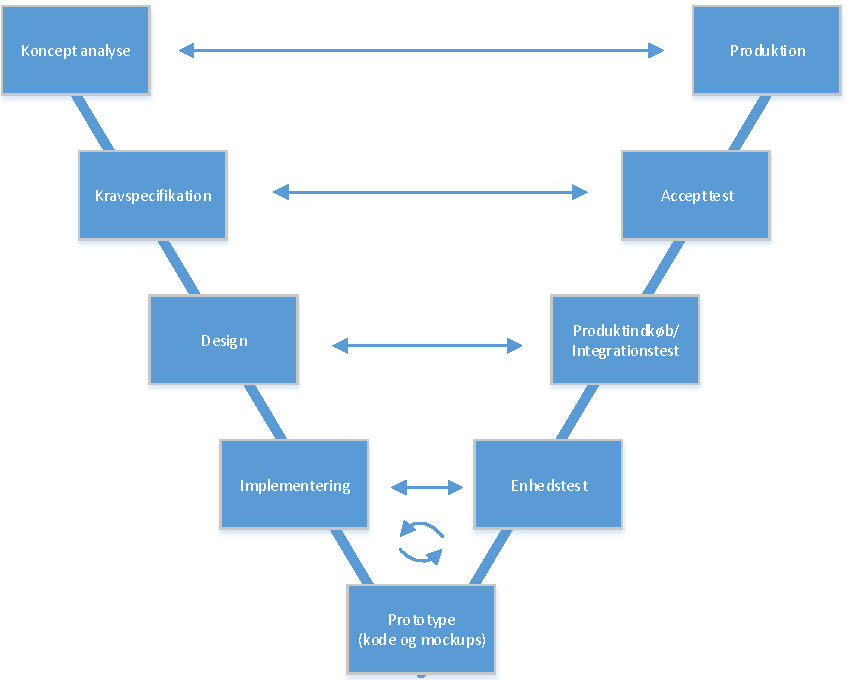
\includegraphics[width=0.7\textwidth]{billeder/Hovedrapport/V-model.PDF}
	\caption{V-model}
	\label{fig:v-model}
\end{figure}

I modsætning til v-modellen findes vandfaldsmodellen, hvor hver enkelt fase bliver lavet færdig før næste fase påbegyndes. Dette medfører ofte nedprioritering af test og andre sene deadlines i projektet, grundet at tidligere tidsplaner er overskredet. Det er derfor denne type model ikke er anvendt i projektet.
\newpage

\section{Første udviklingsfase: Konceptanalyse}
For at eftervise at der er brugt de beskrevne metoder ovenfor, er der valgt at tage eksempler med i rapporten. I afsnittet er der eksempler fra hver af de fire udviklingsfaser. Den første fase er konceptanalysen, som primært har bestået af udarbejdning af forprojektet. I forprojektet er der kort defineret krav, bdd samt en projektplan for projektet. Projektplanen i koncept analysen kan ses på figur \ref{fig:forprojekt}

\begin{figure}[H]
	\centering
	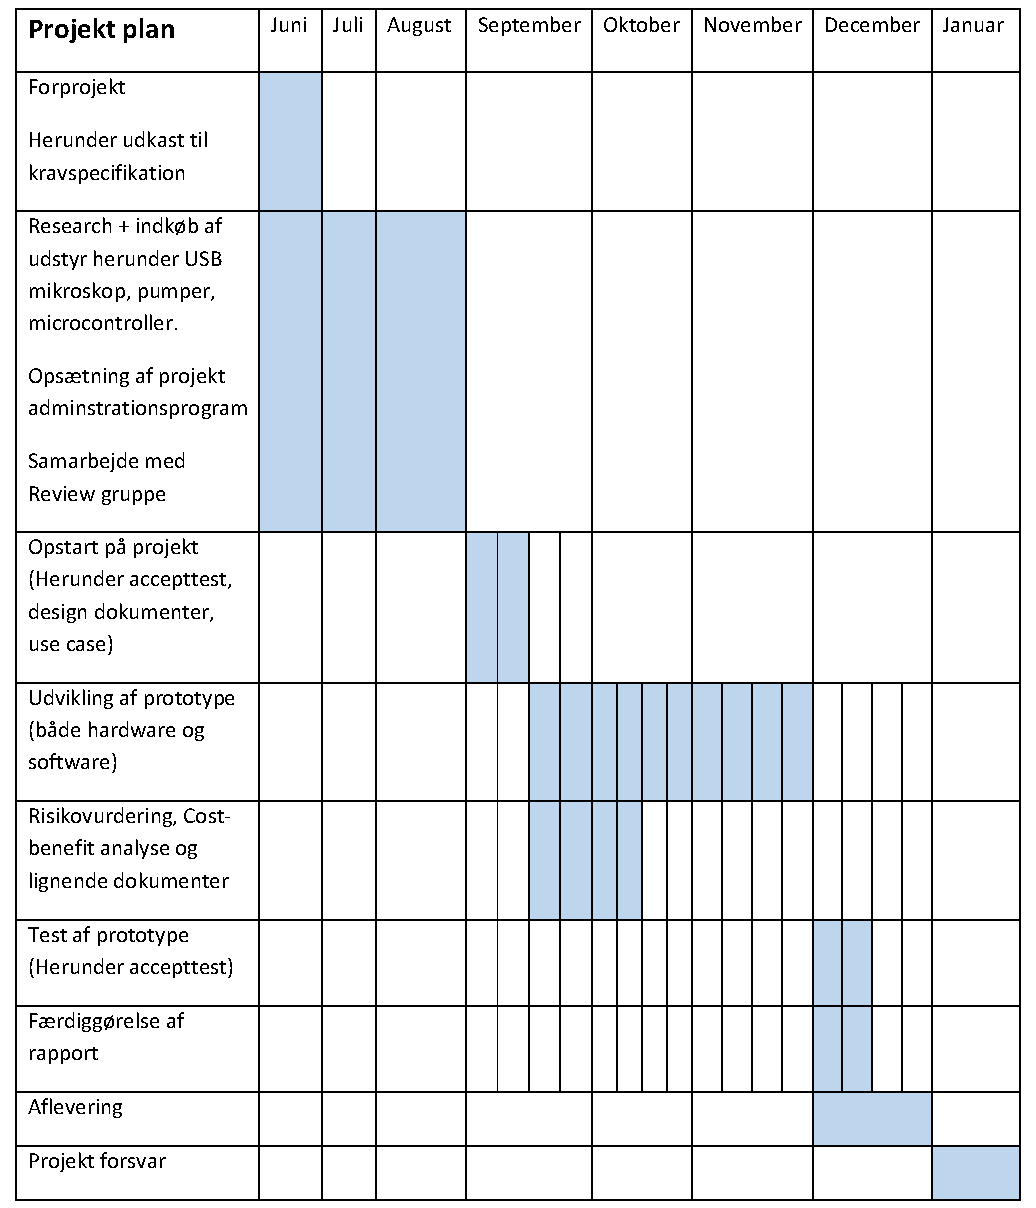
\includegraphics[width=0.9\textwidth]{billeder/Hovedrapport/forprojektplan.pdf}
	\caption{Projektplan i forprojektet}
	\label{fig:forprojekt}
\end{figure}
Det er blandt andet projektplanen på figur \ref{fig:forprojekt}, som har henledt til stage gate modellen. Til sidst har konceptanalysen været med til at give et overblik over hvilke komponenter, der kunne være anvendelige og burde undersøges til prototypen.
 
\section{Anden udviklingsfase: Kravspecifikation og accepttest}
\label{subsec:krav}
For at vise et eksempel for den anden udviklingsfase i projektet, er der valgt at tage \textit{Aktør beskrivelse}, \textit{use case diagram}, samt et \textit{fully dressed use case} og et udpluk fra accepttesten.


\subsection{Aktør beskrivelse}
Systemets primære aktør er operatøren, som står for påfyldning af celler, samt start og stop af sorteringsprocessen. Operatøren har mulighed for at interagere med systemet via en grafisk brugergrænseflade. Systemets sekundære aktør er kameraet og PC’ens filsystem. Kameraet er systemets interface til detektion af de langerhanske øer. Filsystemet er hvor der gemmes en log over sorteringsprocessen.
\newpage
\subsection{Use case Diagram}
I Use case diagrammet (figur: \ref{fig:usecase}) er der vist, hvilke use cases systemet \textit{The Cell Collector} består af. Yderligere er det vist, hvilke aktører der initierer de enkelte use cases. På venstre side er systemets primære aktør \textit{operatøren} vist, mens systemets sekundære aktører \textit{kamera} og \textit{database} er placeret i højre side. 

\begin{figure}[H]
	\centering
	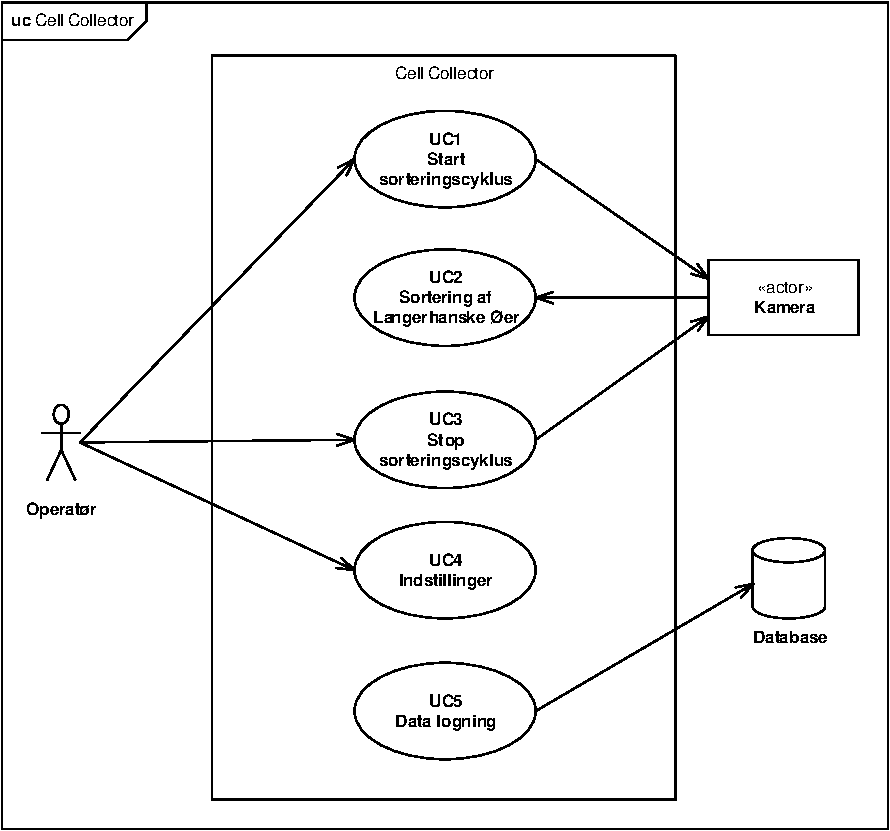
\includegraphics[width=1\textwidth]{billeder/UC_CellCollector.pdf}
	\caption{Use Case diagram for The Cell Collector}
	\label{fig:usecase}
\end{figure}

Efter use case diagrammet var færdigt, blev der udarbejdet fully dressed use cases, som er vist på nedenstående tabel. Tabellen beskriver normalforløbet og undtagelser for \textit{Start af sorteringscyklus}. 

\newpage 
\subsection{Fully dressed use case for use case 1}
\begin{center}
		\begin{longtable}{ | m{4cm} | m{8cm}| } 
			\hline
			Mål & Start sorteringscyklus \\ 
			\hline
			Initiering &  Use casen initieres af operatøren\\
			\hline
			Aktør & 
			Primær: Operatør
			
			 Sekundær: Kamera			  \\ 
			\hline
			Startbetingelser & The Cell Collector programmet er startet på computeren \\ 
			\hline	
			Slutbetingelser ved succes & Systemet starter med sorteringen af Langerhanske øer \\
			\hline
			Slutbetingelser ved undtagelse & N/A \\
			\hline
			Normalforløb & \begin{enumerate}
				%\setlength\itemsep{0cm} % Decrease line distance
				\item Operatør fylder celleopløsningsbeholderen
				\item Celleopløsningsbeholderen er fyldt
				\item Operatør starter sorteringscyklus ved at klikke på [Start]
				\subitem [Undtagelse 1: Wastebeholder er fyldt] 
				\item Systemet initialiserer Arduinoen
				\subitem [Undtagelse 2: Ingen forbindelse til Arduino]
				\item Systemet kontrollerer celleopløsningsbeholderen ved at konvertere spændingen (\SI{}{\volt})  til \SI{}{\milli\litre}, og vise beholderens indhold (\SI{}{\milli\litre}) på GUI
				\item Systemet initialiserer kameraet
				\subitem [Undtagelse 3: Kameraet initialiserer ikke]
				\item Systemet tænder for kamera lyset
				\item Systemet tænder for pumpen
				
			\end{enumerate} \\ 
			\hline
			Undtagelser & [Undtagelse 1: Wastebeholder er fyldt] 
			
			\begin{enumerate}
			\item Systembesked: Tøm venligst Wastebeholder før start
			\item Operatøren trykker “OK”
			\item Systemet fortsætter opstartprocessen
			\end{enumerate} 
			
			[Undtagelse 2: Ingen forbindelse til Arduino]
			
			\begin{enumerate}
			\item 1.	Systembesked: Ingen forbindelse til Arduino, kontrollér forbindelser.
			\end{enumerate} 
	
			[Undtagelse 3: Kameraet initialiseres ikke]
			
			\begin{enumerate}
			\item System fejlmeddelse: Kameraet er ikke initialiseret:
			\item Genstart initialisering af Kameraet
			\end{enumerate} \\
			\hline
		\end{longtable}
		
	\end{center}

Efter at normalforløbet og undtagelserne er defineret, blev accepttesten lavet for den givne use case. Til hvert punkt i normalforløbet er der forberedt en test, som indeholder et \textit{krav nr}, \textit{handling} som beskriver hvad der skal gøres for at starte testen. Derudover er der \textit{forventet resultat}, som skal ske for at testen kan godkendes. \textit{Testmetode} beskriver hvordan testen skal udføres og hvordan den godkendes. Denne test er et udsnit af accepttesten, som er udarbejdet i samarbejde med kunden.

\subsection{Accepttest for krav 1.3}
	\begin{center}
		\begin{longtable}{ | m{4cm}| m{8.5cm}|} 
			\hline
			\textbf{Krav nr.} & 1.3    \\ 
			\hline
			\textbf{Handling} &  Operatør starter sorteringscyklus ved at klikke på [Start]  \\
			\hline
			\textbf{Forventet resultat} &  Opstartsprocessen igangsættes.  \\
			\hline
			\textbf{Testmetode}  & Knappen [Start] trykkes, observeres ved tekstboks på GUI, med teksten \textit{systemet starter op}.   \\
			\hline
			\textbf{Resultat}  &    \\
			\hline
			\textbf{Angiv godkendelse} &     \\
			\hline
			\textbf{Initialer} &     \\
			\hline
			\textbf{Dato} &    \\
			\hline
		\end{longtable}
	\end{center}
	
Resten af accepttesten for use casene kan ses i projektdokumentationen afsnit 2.2.

\section{Tredje udviklingsfase: Design}
\label{subsec:design}
I dette afsnit er der givet et eksempel på, hvordan projektet er gået fra krav til måder at løse projektet på. Der er blandt andet brugt BDD, IBD, flowchart samt sekvensdiagrammer til at beskrive funktioner og sammenhænge i projektet. 

\subsection{BDD og IBD for hardware}
Block definition diagram og interal block diagram over hardwaren er i projektet brugt til at sikre, hver hardware element kan kommunikere med hinanden. Yderligere er det med til at definere specifikationerne, for eksempelvis at indskærpe antallet af strømforsyninger.

Nedenstående BDD \ref{fig:bdd_Hardware} giver et overordnet overblik i, hvad \textit{The cell collector} indeholder af hardware elementer. Hierarkiet starter øverst med \textit{The cell collector}, som indeholder tre mindre hardware dele. Styreenheden, der er defineret som Arduino, indeholder bl.a. underelementet motordriver. Motordriveren indeholder yderligere tre dele,  det vil sige at pumpen, ventilen og kameralyset bliver styret her igennem. Udover styreenheden er der ikke elektriske dele, som beholdere og føringsveje til opløsningen med langerhanske øer. Den tredje underblok til \textit{The cell collector} er kameraet.

\begin{figure}[H]
	\centering
	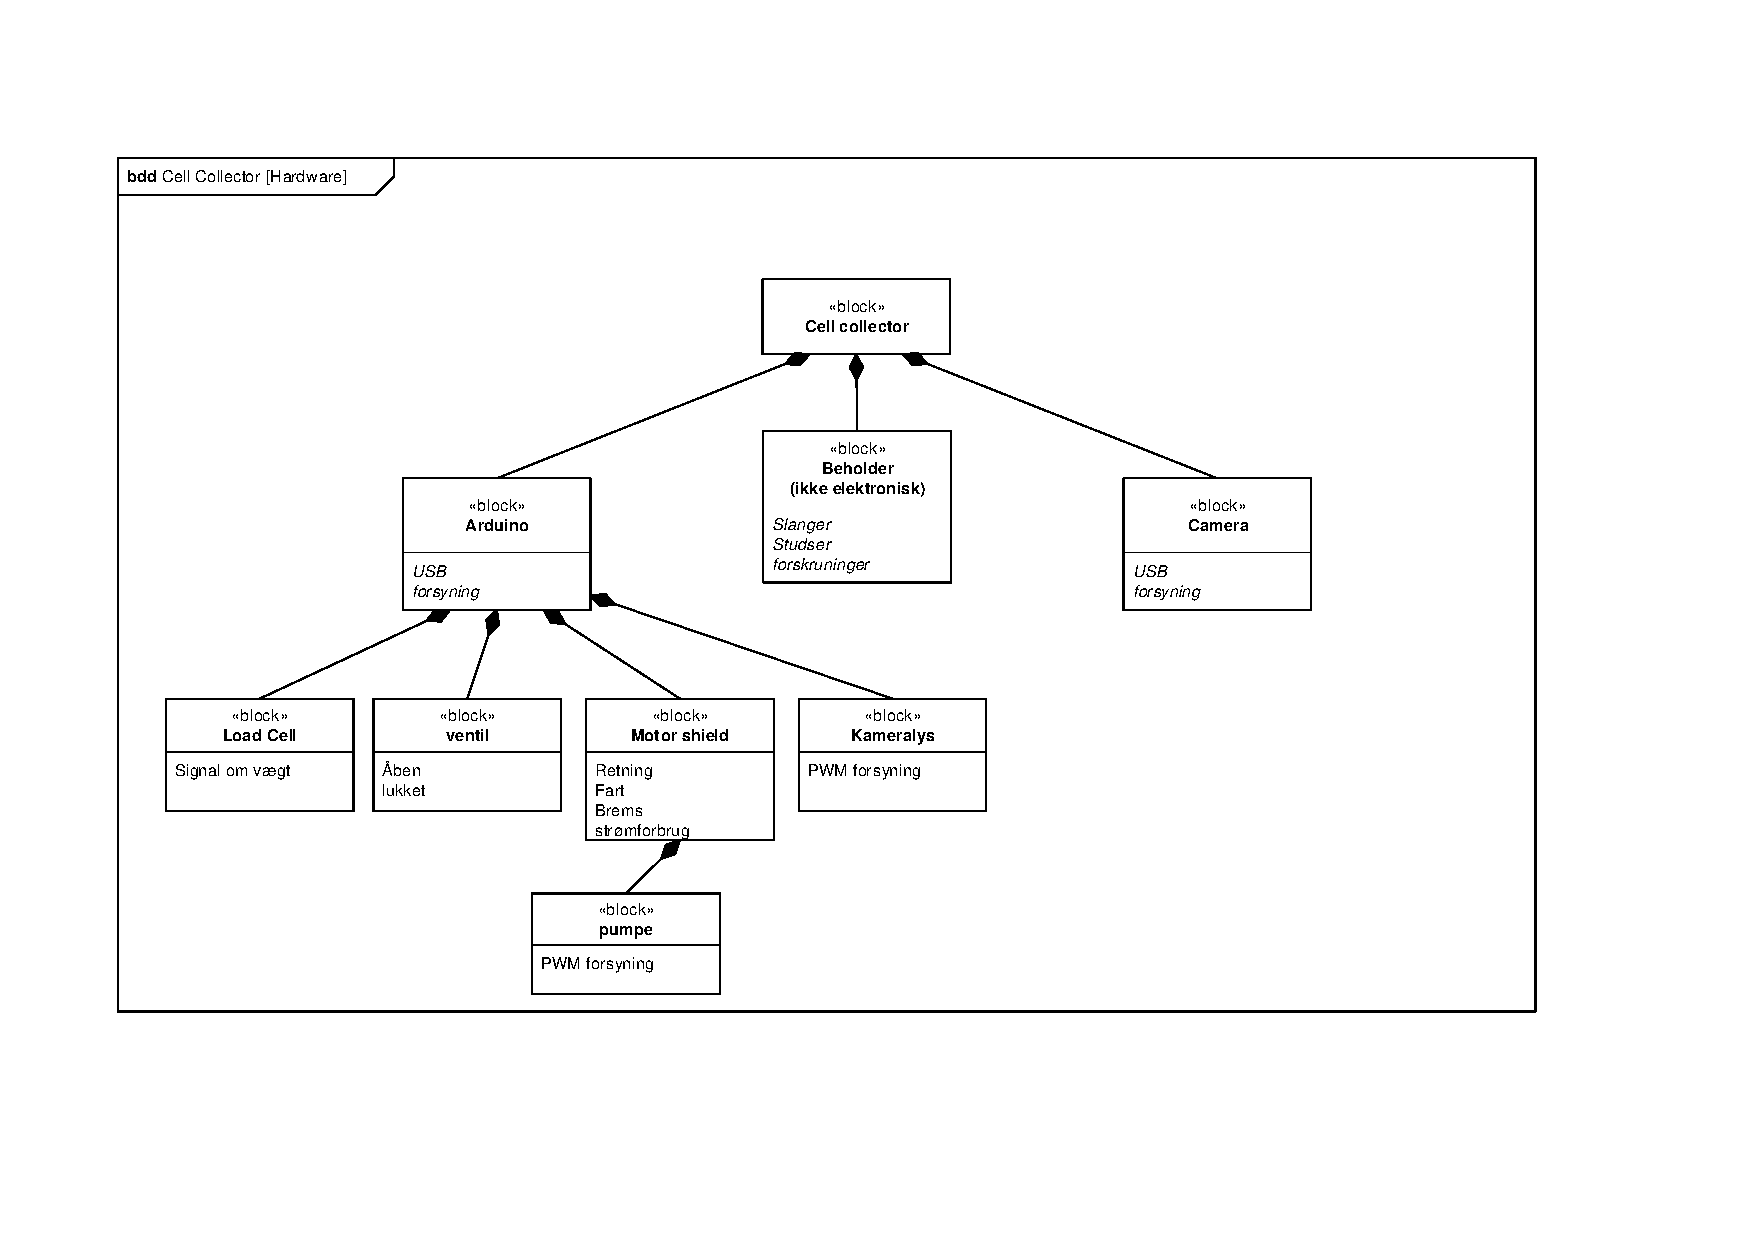
\includegraphics[width=1\textwidth]{pdf/BDD_Hardware.pdf}
	\caption{BDD - Cell Collector [Hardware]}
	\label{fig:bdd_Hardware}
\end{figure}

Nedenstående IBD figur \ref{fig:ibd_Hardware} beskriver mere præcist, hvordan de forskellige komponenter interagerer med hinanden. Diagrammet er brugt til, at der tidligt i udviklingsforløbet bliver defineret hvilke spændinger og signaltyper systemet skal indeholde. Systemet skal indeholde bestemte typer for, at kunne kommunikere med de interne dele.


\begin{figure}[H]
	\centering
	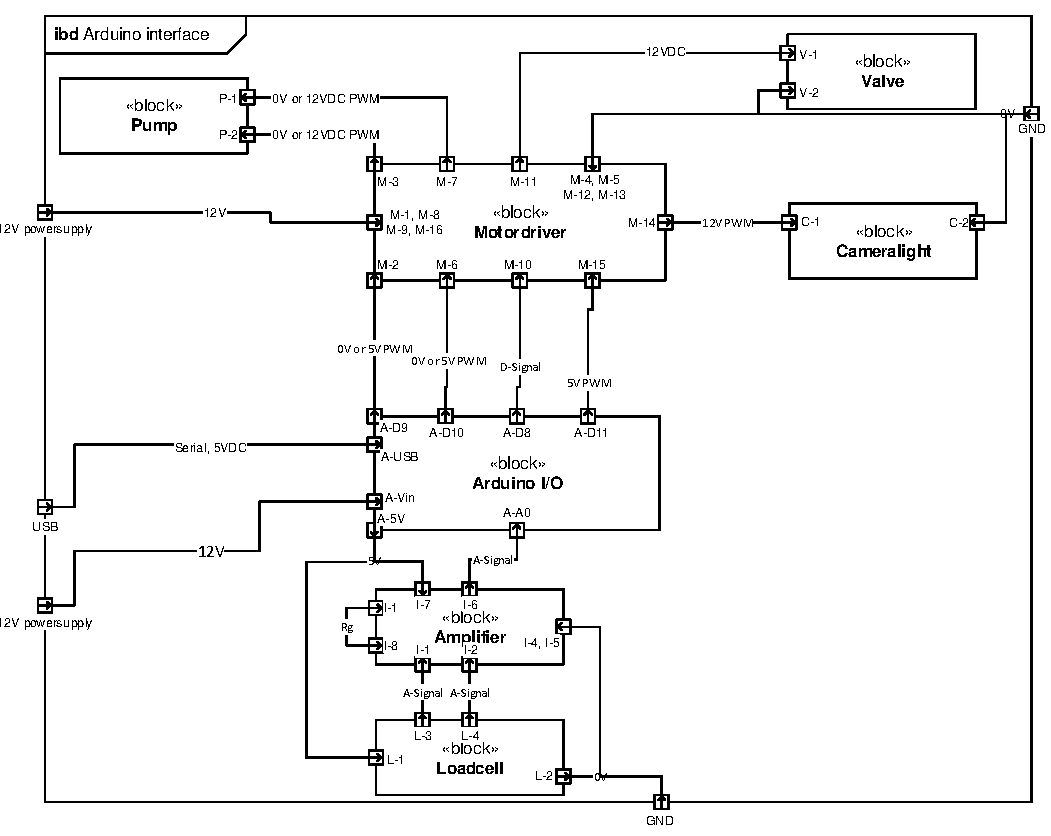
\includegraphics[width=1\textwidth]{pdf/IBD_Hardware(Arduino).pdf}
	\caption{IBD - Cell Collector [Hardware]}
	\label{fig:ibd_Hardware}
\end{figure}

Til ovenstående diagrammer er der udarbejdet tabeller som beskriver signalerne og de enkelte blokke (Se projektdokumentationen afsnit 3.3.4). 

I designfasen er der udarbejdet specifikationer for de enkelte hardware dele, samt overvejelser omkring komponenten. 
\newpage
\subsection{Sekvensdiagrammer}
I designdokumentet er der yderligere lavet sekvensdiagrammer, hvilet giver overblik over de sekventielle dele af systemet til hver use case (se figur \ref{fig:sekvendisgr} for et eksempel). Sekvensdiagrammerne har været brugt til at klargøre, hvordan softwaren skal implementeres og i hvilken rækkefølge funktionerne skal eksekveres. Derudover har det været med til at danne et overblik over delene, der skal implementeres i projektet, samt dele arbejdsopgaverne op i mindre opgaver.
\begin{figure}[H]
	\centering
	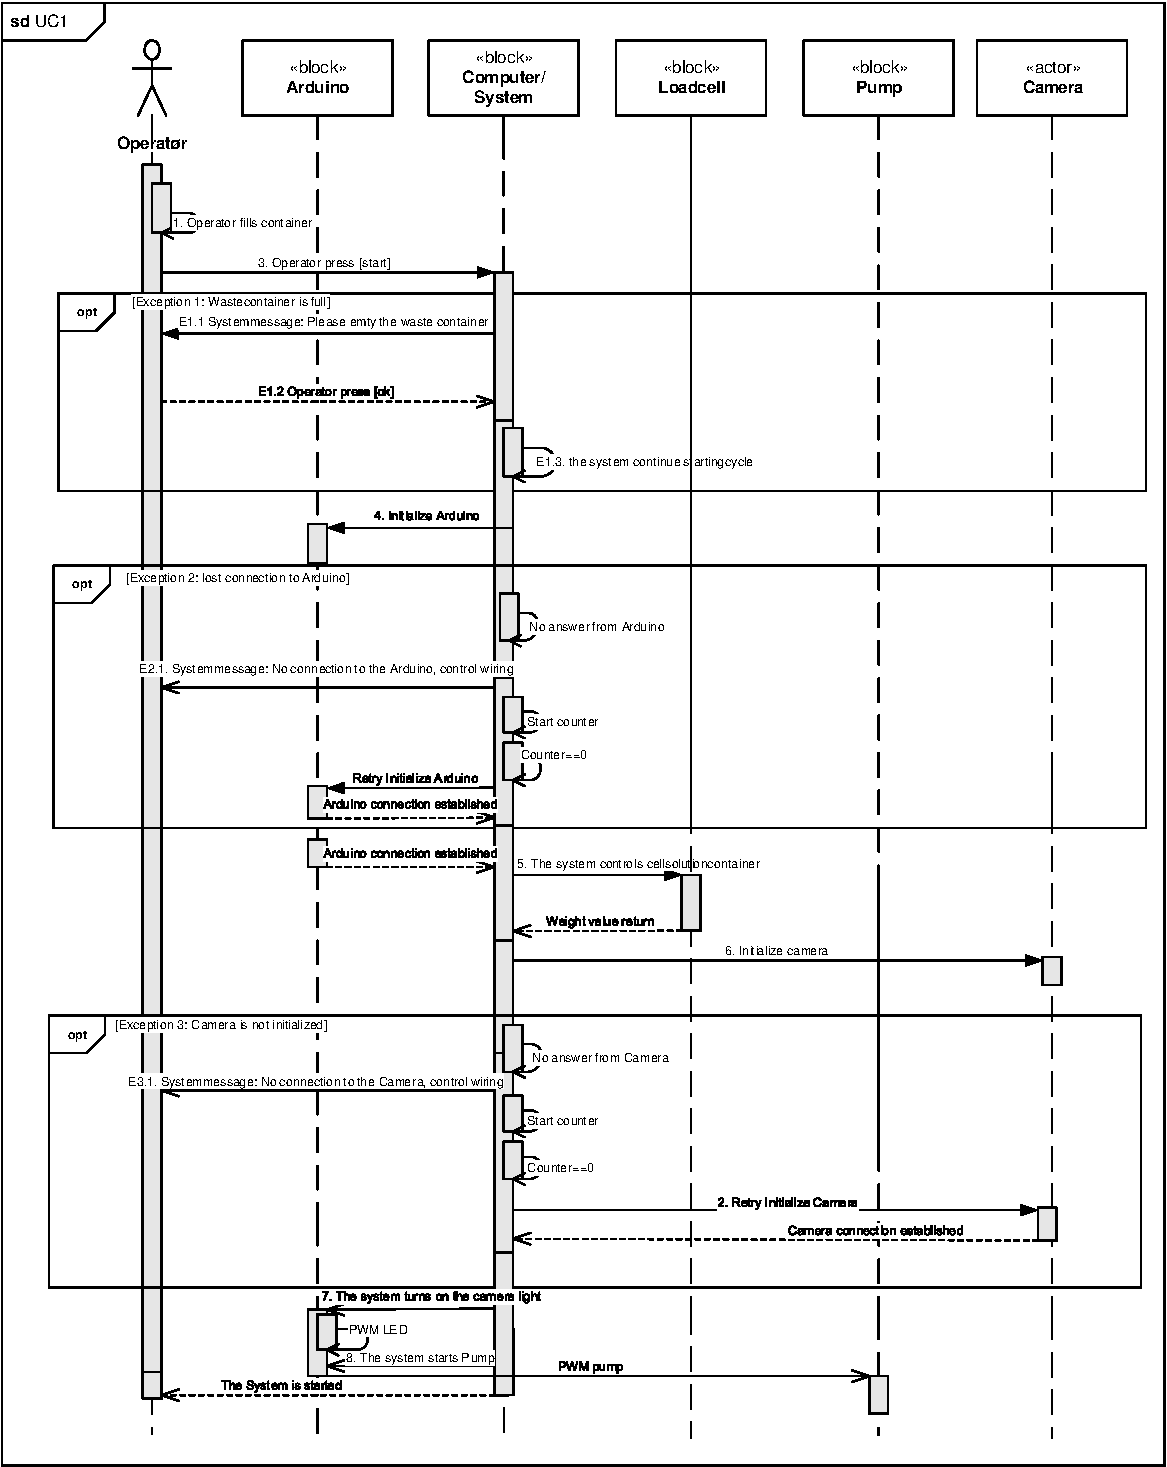
\includegraphics[width=1\textwidth]{pdf/UC1_cropped.pdf}
	\caption{Sekvensdiagram for usecase 1}
	\label{fig:sekvendisgr}
\end{figure}


\subsection{Vægtcelle}
Det følgende afsnit er et eksempel på, hvordan de enkelte hardware komponenter er blevet specificeret i designdokumentet, herunder de overvejelser, der er gjort. Afsnittet viser, hvordan vægtcellen er specificeret.

\label{subsec:loadcell}
Vægtcellen skal bruges til at kontrollere om, der er væske i celleopløsningsbeholderen. Systemet stopper sin sorteringscyklus, når der ikke længere er væske i celleopløsningsbeholderen.

\textbf{Specifikationer for Vægtcelle[\citet{DH7}]:} 
\begin{center}
		\begin{longtable}{ | m{6.5cm} | m{6.5cm}| } 
			\hline
			\textbf{Specifikation} &\textbf{Værdi} \\ 
			\hline
			\textbf{Max belastning:} & 1 kg \\ 
			\hline
			\textbf{Anbefalet arbejdsspænding} & 3-12V \\ 
			\hline
			\textbf{Output} & 1.0mV/V$\pm$0.15mV/V \\ 
			\hline
		\end{longtable}
\end{center}

Den indkøbte vægtcelle kan veje op til 1 kg, hvilket dækker vægten for celleopløsningsbeholderen på 250ml + beholderens vægt. I designfasen er der udarbejdet et teoriafsnit for at dokumentere den opnåede viden gruppen har fået. Designafsnittet indeholder desuden beregninger og kredsløbsdiagrammer. Det er illustreret i den overstående tabel, at vægtcellens output er i millivolt, hvilket har medført, at signalet skulle forstærkes. Dette er gjort vha. en operationsforstærker. For at vise et eksempel, er der trukket nedenstående afsnit ud fra designdokumentet (se projektdokumentation afsnit 3.3.8  for hele afsnittet). I databladet \ref{bilag:INA114} til INA114 vises det at operationsforstærkeren har en CMRR på 115dB, ved et gain på 1000 og en indgangsmodstand på 10G$\Omega$. Forstærkningen kan regnes ud fra formlen i databladet \ref{eq:gainina1}
\begin{align}
 G=(1+\frac{50K\Omega}{R_{G}})
 \label{eq:gainina1}
 \end{align} 
 I dette projekt skal der bruges et gain på $\frac{4,9V}{5mV}=980$. De  4,9V er for ikke at komme i mætning på Arduinoens ADC og 5mV er den maksimale spænding vægtcellen kan give, ved 5V forsyning.
 \begin{align}
 R_{G}=\frac{50k\Omega}{980-1}=51\Omega
 \label{eq:gainina2}
 \end{align}
Et gain på 980 giver en $NY_{Maksimalespænding}=980*5mV=4,9V \pm0,147V$, dvs at der nu er en opløsning på
\begin{align}
 \frac{1000g}{trin}=\frac{1000g}{1024}=0,977g/trin=>0,977*\frac{1024}{5V}=200g/V \pm30g
 \label{eq:gainina3}
 \end{align}
 
 Kredsløbet for INA114 og vægtcellen til Arduinoen er vist på figur \ref{fig:loadcelldiagram}.
 
  \begin{figure}[H]
	\centering
	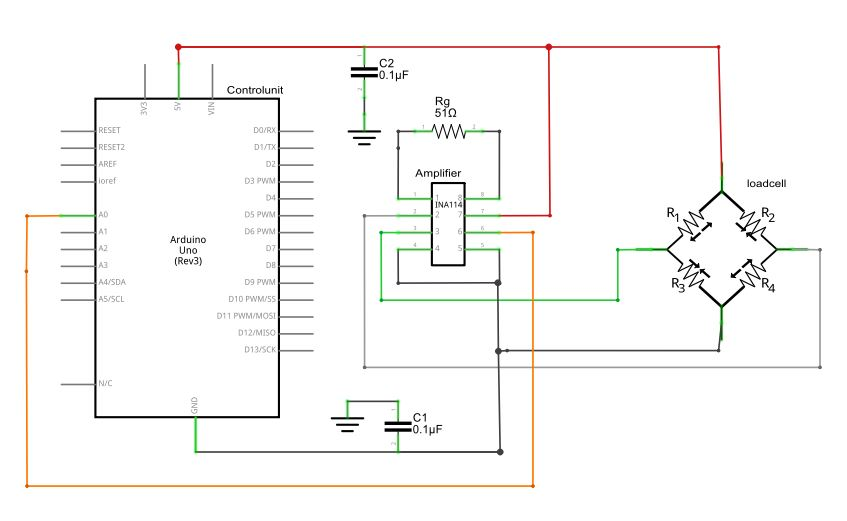
\includegraphics[width=0.9\textwidth]{billeder/Hardware/diagrammer/loadcelldiagram.JPG}
	\caption{Kredsløb for Arduino, INA114 og vægtcelle}
	\label{fig:loadcelldiagram}
\end{figure}



\newpage
\section{Fjerde udviklingsfase: Implementering og enhedstest}
\label{subsec:Implement}
I dette afsnit er der vist et eksempel på hvordan vægtcellen er implementeret, både hardware- og softwaremæssigt. Til sidst i implementeringsfasen er der lavet en integrationstest. Integrationstesten for hardwaren er bestået i udarbejdelse af et shield til \textit{Arduinoen}. Da de enkelte faser er foregået ved en iterativ proces har det været mulighed at justere designdokumentet, hvis en komponent eller funktion blev implementeret anderledes end det var specificeret. På samme måde er designdokumentet ændret, hvis en enhedstest fejlede. Et eksempel på dette er kameraet, hvor det i enhedstesten viste sig at kvaliteten ikke var tilstrækkelig. Enhedstesten for kameraet er vist i afsnit 4.3.1 i projektdokumentation. 

\subsection{Hardware}
Efter at diagrammet og kredsløbet er fastlagt i designdokumentet kunne vægtcellens kredsløb nu testes på et \textit{fumlebræt}. Se figur \ref{fig:loadcelltest} for testopstilling.

  \begin{figure}[H]
	\centering
	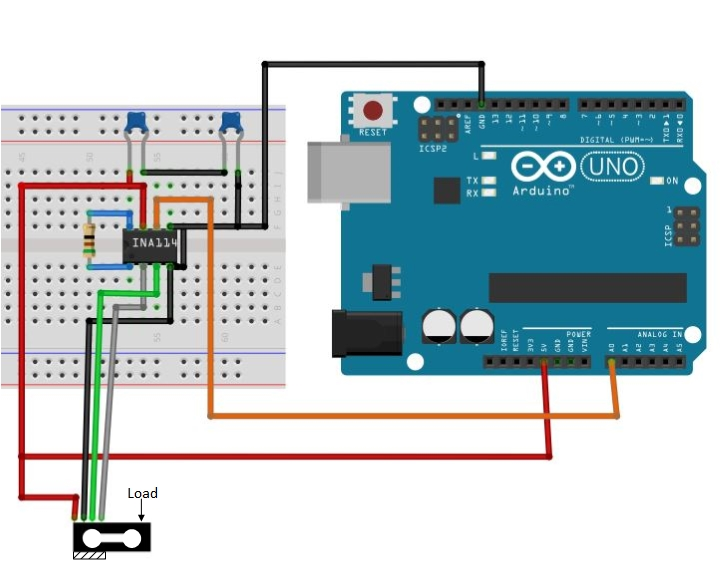
\includegraphics[width=0.9\textwidth]{billeder/Hardware/diagrammer/Drawing1.jpg}
	\caption{Test opstilling for vægtcelle}
	\label{fig:loadcelltest}
\end{figure}
De primære dele af test koden har været  \textit{sensorValue = analogRead(A0);} og \textit{Serial.println(sensorValue);}, hvor ved at inputtet på \textit{A0} er læst i \textit{serial monitor}, som vist på figur \ref{fig:loadcell_test} ved langsom tømning af beholderen.

\begin{figure}[H]
	\centering
	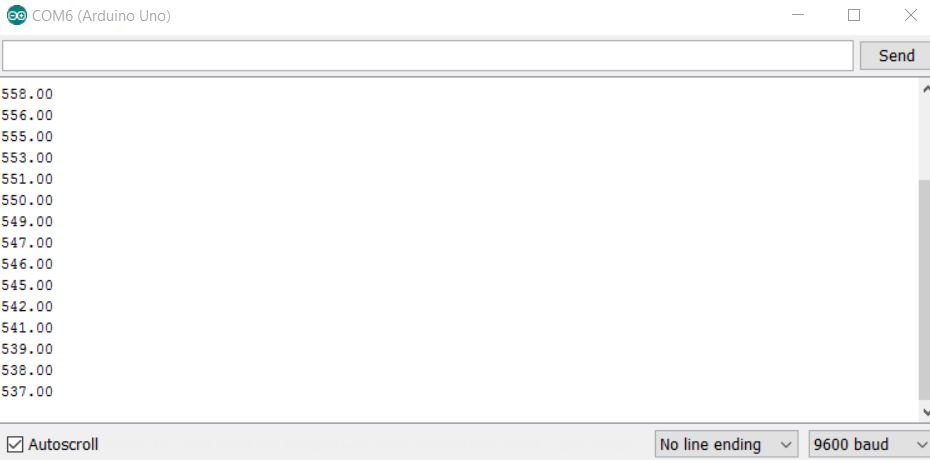
\includegraphics[width=0.9\textwidth]{billeder/Hardware/diagrammer/loadcellunittestbits.JPG}
	\caption{Værdier fra A0 i \textit{serial monitor}}
	\label{fig:loadcell_test}
\end{figure}

 Se bilag \ref{bilag:TKloadcell} for at se hele koden til testen. Til enhedstesten er der brugt et voltmeter til at måle udgangsspændingen på INA114 for at se, om Arduinoens ADC læste rigtigt. Til at sammenligne med voltmeteret, blev formlen \ref{eq:trintilvolt} brugt til at konvertere ADC'ens bits værdi om til spænding.
 
 \begin{align}
 analogRead(A_0)*\frac{5}{1024}=\text{spænding i volt}
 \label{eq:trintilvolt}
 \end{align}
Testopstilling af vægtcellen ser ud som på figur \ref{fig:loadcell_mont} med celleopløsningsbeholderen. I softwaren kræves det en kalibrering for at vægtcellen er præcis, dette er implementeret i projektdokumentation afsnit 4.3.4.5.
 
 \begin{figure}[H]
	\centering
	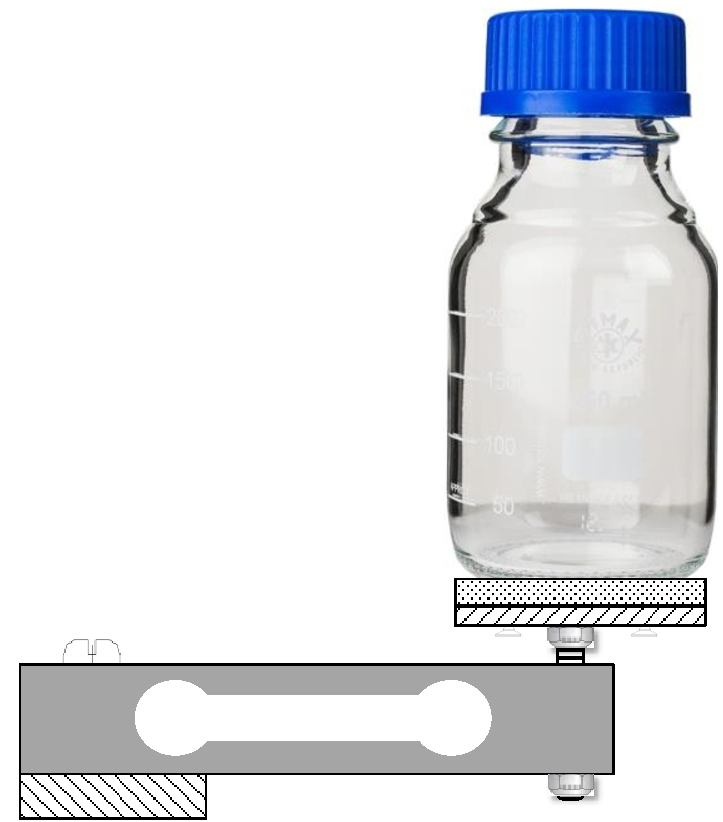
\includegraphics[width=0.5\textwidth]{billeder/Hardware/diagrammer/loadcell_montering.pdf}
	\caption{Illustration af opstilling med vægtcelle og celleopløsningsbeholder}
	\label{fig:loadcell_mont}
\end{figure}

\subsection{Kalibrering af vægtcellen}
Funktionen til vægtcellen er implementeret efter beskrivelsen i designdokumentet i projektdokumentation afsnit 3.4.1.1. Dens funktion er at konvertere det analoge input (V) til indholdet (ml) i celleopløsningsbeholderen. Dette er implementeret ved en lineær model:
\begin{align}
mL = a*input+b \text{, hvor a er hældningen og b er skæringen med y aksen}
\end{align}
Det analoge input ganges med en faktor \textit{a} plus et offset \textit{b} for at konvertere spænding til antal ml. Nedenstående tabel viser indgangsspændingen for forskellige mængder i beholderen. Udfra disse data er der lavet en lineær regression for at finde hældningen \textit{a} og skæringen \textit{b}.
\begin{center}
		\begin{longtable}{ | m{3cm} | m{3cm}| } 
			\hline
			\textbf{ml i beholder} &\textbf{Analog input} \\ 
			\hline
			 \SI{0}{\milli\litre} & \SI{1.9487}{\volt} \\ 
			\hline
			 \SI{25}{\milli\litre} & \SI{2.0440}{\volt} \\ 
			\hline
			\SI{50}{\milli\litre} & \SI{2.1320}{\volt} \\ 
			\hline
			\SI{75}{\milli\litre} & \SI{2.2297}{\volt} \\ 
			\hline
			\SI{100}{\milli\litre} & \SI{2.3109}{\volt} \\ 
			\hline
			\SI{125}{\milli\litre} & \SI{2.4071}{\volt} \\ 
			\hline
			\SI{150}{\milli\litre} & \SI{2.4961}{\volt} \\ 
			\hline
			\SI{175}{\milli\litre} & \SI{2.5821}{\volt} \\ 
			\hline
			\SI{200}{\milli\litre} & \SI{2.6760}{\volt} \\ 
			\hline
			\SI{225}{\milli\litre} & \SI{2.7654}{\volt} \\ 
			\hline
			\SI{250}{\milli\litre} & \SI{2.8587}{\volt} \\ 
			\hline
			\caption{Kalibreringsdata for vægtcellen}
			 		\end{longtable}
\end{center}

I Matlab er funktionen \textit{fitlm} anvendt til at finde det bedste lineære fit. Regressionen er baseret på Least Square metoden \citep{least}.
Udfra beregningerne i Matlab er hældningen a og skæringen b fundet til hhv:
\begin{align}
a = 276.14
\end{align}
\begin{align}
b = -539.02
\end{align}
Den endelige funktion er givet ved:
\begin{align}
ml = 276.140*input-539.02
\end{align}

Figur \ref{fig:loadcellcalib} viser den lineære funktion, samt de enkelte data punkter fra tabellen. 
\begin{figure}[H]
	\centering
	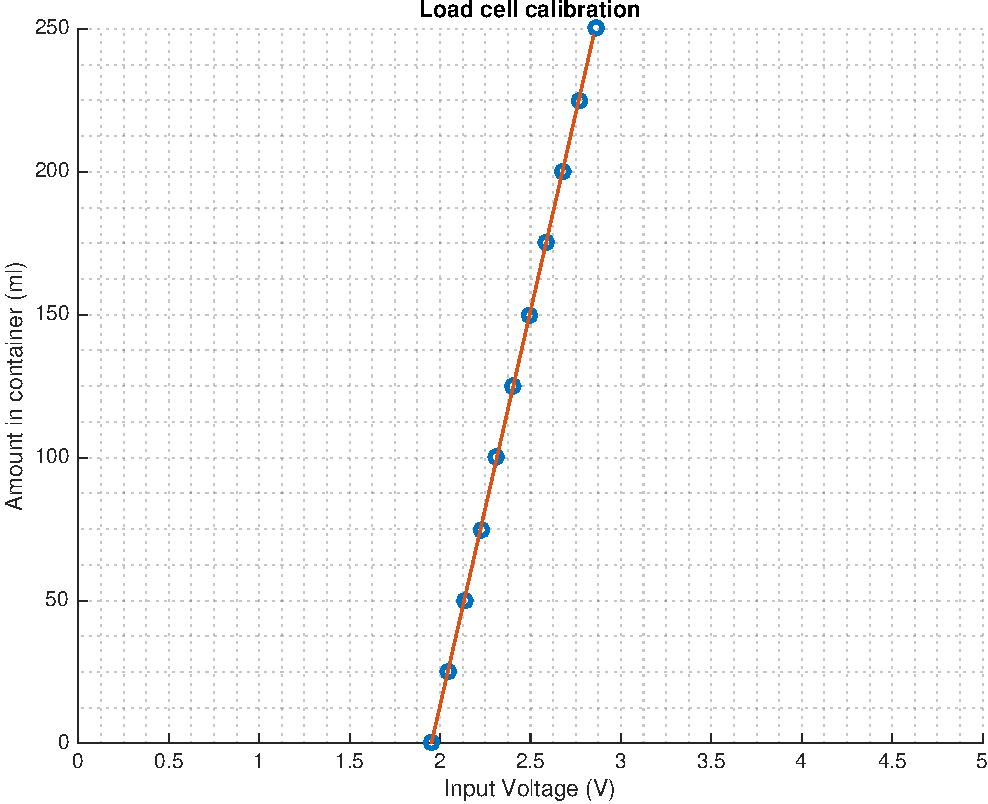
\includegraphics[width=0.6\textwidth]{billeder/software/calibration-crop.pdf}
	\caption{Kalibrering af load cell}
	\label{fig:loadcellcalib}
\end{figure}

For at reducere støj og mindske følsomheden overfor hurtigere ændringer i indgangsspændingen er der implementeret en midling af de seneste 10 målinger. Dette er med til, at gøre konverteringen mere robust overfor støj. 


\subsection{Integrationstest}
Til sidst i denne fase er der udført en integrationstest, hvor hardwaren er samlet, efter alle enkelte enhedstest er udført. Efter samlingen af hardwaren er det verificeret at kredsløbet virker, hvorefter der er designet et PCB til samlingen af hardwaren. Før integrationstest med hardwaren blev softwarens interface med Arduinoen testet vha. LED'er. Lysdioderne er brugt til at koble på de udgange hvor ventil, pumpe og kameralys skal monteres. Dette gav mulighed for visuelt at se om udgangene på Arduinoen blev sat høj(5V) og lav(0V) som forventet. Herudover blev et potentiometer brugt, som erstatning til vægtcellen. Dermed kunne indgangsspændingen manuelt justeres og det kunne dermed visuelt observeres at beholderens indhold blev ændret.
Til sidst i integrationstesten blev de egentlige hardware komponenter koblet på Arduinoens porte og det blev testet om softwaren fortsat kørte efter hensigten.


\chapter{Resultater}

\section{Det færdige system}
- Kamera

\section{Cost-benefit analyse}
Økonomisk

Andre ting?
\chapter{Perspektivering}
Dette kapitel indeholder perspektivering af projektet, som kan udføres i en videreudvikling af projektet.
\section{Kamera}
 I en videreudvikling af projektet bør der laves en test af en række forskellige kameraer for, at denne del af systemet har en tilstrækkelig kvalitet. Dermed kan kvaliteten af kameraerne testes inden et bestemt kamera indkøbes. Testen skal foretages ved, at der tages en række billeder af langerhanske øer, ideelt hvor øerne pumpes i gennem slangen for at komme tæt på brugsscenariet. 

\section{Påvirkning af langerhanske øer}
I et senere stadie af projektet bør der undersøges, hvor meget tryk og stress de langerhanske øer kan tåle. Området indeholder mange faktorer der stadig er ukendte, hvilket bør undersøges. Derfor kræves et mindre studie omkring dette. Metoden det kan gøres på er ved at teste, hvor meget insulin øerne producerer efter, at de har været påvirket på forskellige måder. På den måde kan de isolerede øer testes inden og efter, at de pumpes igennem systemet, hvorefter  resultatet sammenlignes. Det skal blandt andet undersøges, hvordan øerne opfører sig ved en peristaltisk pumpe, som brugt i projektet. Derudover bør ventilen undersøges. Hvis testen giver negative resultater bør systemet deles op, for at teste pumpen og ventilen hver for sig.

\section{Pumpe}
Den peristaltiske pumpe virker ved at sammenpresse slangen med roterende ruller, hvor slangen efter sammenpresningen udvider sig  og dermed trækker væsken til sig. Væsken indespærres af den næste rulle, som sammenpresser slangen, og væsken drives derfor ud af slangen. Fordelene ved en peristaltisk pumpe er, at væsken ikke forurenes, da væsken er isoleret fra pumpen vha. slangen. Derudover skabes der et præcist flow og pumpen kan ikke løbe "tør"  da den er selvspædende. Ulempen ved en peristaltisk pumpe er, at den netop sammenpresser slangen, hvilket kan risikere at klemme på de langerhanske øer. For at forhindre, at øerne bliver beskadiget kan en sprøjtepumpe overvejes, fordi der bør være mindre påvirkning af øerne. Det vil være ideelt hvis der et konstant flow med henblik på, at opnå kravet om de 30 isolerede øer i minuttet. Derfor kan en tocylindret sprøjtepumpe med tilhørende ventiler bruges, for at holde hastigheden konstant. 

\section{Ventil}
Ved ventilen skal der undersøges, hvor lang tid der går fra kameraet har detekteret en langerhanske ø til den er ved ventilen. I projektet er forsøget kun lavet med simuleringsvæsken, men sandsynligheden for, at de langerhanske øer har samme væskeegenskaber som frøene brugt i simuleringsvæsken, er forholdsvis lav. Det er derfor ikke sikkert at tidsintervallet er det samme. Grunden til at forsøget bør laves er, at det er vigtigt, at ventilen isolerer de langerhanske øer, men det er heller ikke anvendeligt, at få for meget eksokrint væv med. Yderligere vil et mindre volumen i ventilen være favorabel, for at gøre udtømningstiden af ventilen mindre.   

\section{Parallelle systemer}
For at opnå en højere hastighed, kan parallelle rør systemer ført forbi kameraet overvejes.
Da kameraet sandsynligvis har et større synsfelt end én slange, kan systemerne føres forbi det samme kamera. Det kræver dog, at billedprocesseringen er hurtig nok.

\section{Billedprocessering}
I projektet er billederne til billedbehandling simuleret ved at bruge billeder taget af isoleredet øer, hvor der er tilføjet tilfældigt støj og rest væv. I videreudvikling af projektet bør billedprocesseringen optimeres til de faktiske øer i slangen.

\section{Omrøring og køling af celleopløsningsbeholderen}
Til videreudvikling af de ikke-elektroniske dele, bør en omrøring i opløsningsvæsken skabes, da de langerhanske øer bundfælder. Samtidigt bør omrøringen håndteres så skånsomt som muligt så øerne ikke beskadiges. En mulighed kunne være, at den tidligere omtalte sprøjtepumpe roteres, hvor der på den måde vil blive skabt en skånsom omrøring af opløsningsvæsken. Ydermere ville det være at foretrække, hvis systemet kunne nedkøle opløsningsbeholderen, for at sikre at enzymet ikke aktiveres uønsket. Det kunne være bestående af et køle element. 

\section{Medicinsk udstyr}
 Da systemet primært er fokuseret til forskningsbrug, kræver udstyret ikke medicinsk godkendelse. Dog kan systemet på sigt muligvis bruges til ø implantationer, for lindring og som præparat mod diabetes. Skal systemet bruges til dette formål, vil det kræve en medicinsk godkendelse. For at et produkt kan opnå medicinsk godkendelse, skal produktet overholde en række direktiver, som kan opnås igennem harmoniseret standarder. Det første punkt ved medicinsk godkendelse er udstyrets formål (intended use), da det er formålet der styrer klassifikationen for udstyret. I Europa klassificeres der efter 4 klasser I, IIa, IIb og III, hvor klasse III er den med de strengeste krav. Uanset klasse skal udstyret opfylde de væsentlige krav i MDD direktivet, som bl.a. er rapportering af utilsigtede hændelser og overvågning af systemet på markedet. Ydermere skal der foretages en risikoanalyse af produktets risikoer. For at et medicinsk udstyr kan CE mærkes 
 skal det alt efter klassificering, gennemgå trin igennem bilagene i MDD direktivet. Det skal indeholde teknisk dokumentation, væsentlige krav og risikoanalyse. Derudover skal der udarbejdes kvalitetsstyringssystemer til at dokumentere produktets forløb. Dokumentationen skal godkendes af et bemyndiget organ, hvis udstyret vurderes til at være højere end klasse I. Ydermere er der høje krav til versionsstyring af produktet, for at give en gennemsigtig sporbarhed. Før der begyndes på arbejdet med medicinsk godkendelse, er det vigtigt, at intended use klarlægges. Det skal der for at være sikker på, om udstyret går ind under MDD direktivet. Det bør undersøges om produktet kan sammenlignes med en insulinpen, da den går ind under det farmaceutisk direktiv. Det gør den fordi det er insulinen som virker. 
\section{Konklusion}
husk at problemformuleringenspunkter skal kunne afkrydses her nede
%\chapter{Resultater}

\section{Det færdige system}
- Kamera

\section{Cost-benefit analyse}
Økonomisk

Andre ting?
%\chapter{Resultater}

\section{Det færdige system}
- Kamera

\section{Cost-benefit analyse}
Økonomisk

Andre ting?
%\chapter{Resultater}

\section{Det færdige system}
- Kamera

\section{Cost-benefit analyse}
Økonomisk

Andre ting?

%% Afrunding %%

%\section{Konklusion}
husk at problemformuleringenspunkter skal kunne afkrydses her nede


%%%% Kilder %%%%

\begingroup
	\raggedright
	\bibliography{bibtex/litteratur}							% Litteraturlisten inkluderes
\endgroup


%%%% Fixme-listen %%%%

\newpage														% Ny side til Fixme-listen
\listoffixmes													% Fixme-listen - fjernes til sidst i projektet med "%"


%%%% Appendiks %%%%

\appendix														% Appendiks/bilag start - giver chapter bogstaver i stedet for tal
\clearforchapter												% Sikrer at pagestylen aktiveres paa den rigtige side
\phantomsection													% Kunstigt afsnit, som hyperlinks kan 'holde fast i'
\pdfbookmark[0]{Appendiks}{appendiks}							% Tildeler en klikbar bookmark til den endelige PDF

%% Indstillinger for appendiks (deaktiveret med "%") %%

%\pagestyle{empty}												% Sidehoved/-fod for standardsider aendres til tom for appendiks
%\aliaspagestyle{chapter}{empty}								% Sidehoved/-fod for kapitelsider aendres til tom for appendiks
%\settocdepth{chapter}											% Kun kapitel-niveau vises i ToC
%\addtocontents{toc}{\protect\cftpagenumbersoff{chapter}}		% Sidetal for kapitler fjernes i ToC

%% Filer til appendiks %%


%%%% Bilag %%%%

%\phantomsection												% Kunstigt afsnit, som hyperlinks kan 'holde fast i'
%\addcontentsline{toc}{chapter}{Bilag A \ Navn} 				% Manuelle indgange i indholdsfortegnelsen (naar \includepdf bruges)

%\includepdf[pages={x-y}]{filnavn}								% Inkluder eksterne bilag med \includepdf[pages={x-y}]{filnavn}


\end{document}													% Slutter dokumentet - obligatorisk


